% !TEX root = ../HDR.tex
%%%%%%%%%%%%%%%%%%%%%%%%%%%%%%%%%%%%%%%%%%%%%%%%%%%%%%%%%%%%%%%%%%%%%%%%%%%%%%%%%%
\chapter{Ancrage théorique}

\noindent 
Dans leur article \og \an{Universal Intelligence: A Definition of Machine Intelligence} \fg, Shane Legg et Marcus Hutter notent que \og \an{A fundamental problem in artificial intelligence is that nobody really knows what intelligence is} \fg\ \cite[p.~1]{legg_universal_2007}.

Si nous ne savons pas vraiment ce qu'est l'intelligence, nous ne partons quand même pas de zéro. 
Cette question a occupé des nombreux penseurs depuis de nombreux siècles et je crois qu'il est important de savoir nous y référer. 
Ce chapitre vise à définir l'intelligence artificielle précoce telle qu'elle est mise en \oe uvre par les êtres vivants, sur la base de l'épistémologie, la psychologie, des sciences cognitives et des neurosciences. 

La finalité est de fonder un projet d'implémentation informatique qui transcrive cette vision.

\section{Philosophie de l'esprit}
\label{sec:philosophie}

La justification de ce chapitre sur la philosophie de l'esprit est que de nombreux travaux d'intelligence artificielle font référence à des concepts épistémologique. En particulier l'intelligence artificielle fait référence aux épistémologies génétique et constructiviste. 
Il est important de comprendre dans quelle mesure ces travaux reflètent fidèlement ou non ces concepts. 


\subsection{Révolution des Lumières}
\label{sec:lumieres}

\noindent
La révolution épistémologique des Lumières du XVIII\ieme{}~siècle a profondément renouvelé la manière de penser le savoir, la raison et l’expérience.
Dès la fin du XVII\ieme{}~siècle, le philosophe britannique John Locke en fut l'un des précurseurs en fondant \emph{l'empirisme}. 
En rupture avec le rationalisme qui le précédait, Locke élabore une critique décisive de l'innéisme et introduit la célèbre métaphore de la \emph{tabula rasa} pour désigner l’absence de connaissances à la naissance.
L'empirisme remet en cause la notion de vérité indubitable, innée ou issue d'une volonté divine comme dans le cas de Descartes. 
Il affirme que toute connaissance provient de l'\an{experience}, terme anglais qu'il convient d'entendre non pas au sens de \og faire une expérience \fg\ mais au sens \og d'éprouver une expérience \fg, et qu'on trouve traduit en français par \emph{expérience sensible}.

David Hume prolonge et radicalise l'empirisme de Locke en utilisant le terme \an{impression} (\emph{impression sensible}) pour désigner la source des connaissances humaines: 

\begin{quote}
\an{By the term \emph{impression}, I mean all our more lively perceptions, when we hear, or see, or feel, or love, or hate, or desire, or will. [...]
Impressions may be divided into two kinds, those of sensation and those of reflection. The first kind arises in the soul originally, from unknown causes. The second is derived in a great measure from our ideas, and is a result of the mind’s operations.
[...]
What is commonly, in a popular sense, called reason, and is so much recommended in moral discourses, is nothing but a general and a calm passion, which takes a comprehensive and a distant view of its object, and actuates the will, without exciting any sensible emotion.}
\cite{hume_treatise_1739}
\end{quote}

L'empirisme de Hume montre que l'humain est avant tout un être sensible régi par la dynamique complexe et changeante de ses sentiments et passions.  
Il montre la fragilité du lien entre cause et effet : pour lui, la causalité n’est qu’une habitude mentale résultant de la répétition d'impressions.
Il propose la \an{bundle theory} (traduite en français par \emph{théorie du faisceau}, à ne pas confondre avec la \an{sheaf theory} ou théorie mathématique des faiscaux) selon laquelle les objets sont constitués uniquement par une collection (\an{bundle}) d'impressions dont le sujet fait l'expérience.  

Sur le continent européen, le médecin et philosophe français Julien Offray de La Mettrie publie en 1748 \og L'Homme machine \fg\ qui expose une conception résolument matérialiste de l'homme \cite{la_mettrie_homme_1748}.
Il y soutient que la pensée n'est pas le privilège d'une substance immatérielle mais une propriété la \emph{matière organisée}.
Il ne s'agit pas d'une théorie panpsychique qui affirmerait que toute matière possède un certain niveau de conscience; 
le terme matière organisée désigne ici les matières biologiques telle que le cerveau. 
Il formule de manière provocatrice sa thèse moniste: \og Concluons hardiment que l'homme est une machine et qu'il n'y a dans tout l'Univers qu'une seule substance \fg\ qui a été résumée par le slogan \og la matière peut penser \fg .

Au cours de la seconde moitié du XVIII\ieme{}~siècle, Emmanuel Kant critique à la fois le rationalisme du début du XVII\ieme{}~siècle et l'empirisme qui lui a succédé \cite{kant_kritik_1781}.
Tout en reconnaissant la contribution décisive de Hume, il s'en distingue en soutenant que la connaissance ne découle pas passivement de l'expérience mais que le sujet humain organise activement ses expériences.
Il rejette l'idée Lockéenne d'une stricte \emph{tabula rasa}, mais retient de l'empirisme l'idée que la connaissance est limitée par le champ de l'expérience sensible.
Il utilise le terme \emph{phénomène} pour désigner les \og choses en tant qu'elles peuvent être connues par l'Homme à travers l'expérience \fg, et il appelle \emph{noumènes} les \og choses en soi \fg\ inaccessibles à l'expérience et à la connaissance humaine.
Selon lui, toute expérience sensible est déjà conditionnée par les structures du sujet connaissant : les catégories de l'entendement et les formes \textit{a priori} de la sensibilité que sont l'espace et le temps.

Kant se démarque de l'empirisme en considérant que l’esprit occupe un rôle moteur pour structurer les phénomènes à travers des \emph{schèmes} (\an{schemata}).
Les schèmes kantiens servent de médiateurs entre les concepts purs (par exemple causalité, substance, quantité, formes géométriques comme un triangle) et les images sensibles (par exemple un triangle droit ou équilatéral).
Ainsi, le schème de triangle est la règle de construction de tous les triangles possibles dans l'intuition.
La connaissance résulte dès lors de la rencontre entre les données de l’expérience et les formes que l’esprit impose à ces données.

Ces bouleversements du siècle des Lumières ont souligné le rôle fondamental du sujet, la nécessité de l’expérience et la puissance des lois de l’esprit, ouvrant la voie à l'exploration des moyens et des conditions de la connaissance.

\subsection{Théorie de l'évolution}

%Bien que ne portant pas directement sur la philosophie de l'esprit ni sur l'intelligence, il me semble important de mentionner la publication, en 1859, de l'ouvrage de Charles Darwin \og \an{On the origin of species by means of natural selection} \fg.

\noindent
En 1859, Charles Darwin publie son ouvrage \an{On the origin of species by means of natural selection} \fg\ \cite{darwin_origin_1859}.
Cette parution marque un tournant intellectuel dans le prolongement du siècle des Lumières qui inscrit progressivement l’intelligence dans une perspective naturaliste et évolutionniste.
Le philosophe Daniel Dennett soulignera ultérieurement l'ampleur de cette rupture en qualifiant Darwin de \og \an{by far the scientist who has made the greatest contribution to philosophy} \fg\   \cite[p.~10061]{dennett_darwins_2009}.

La théorie darwinienne invite à concevoir les capacités mentales comme le résultat d’un processus d’évolution phylogénétique du vivant, plutôt que comme des facultés abstraites, universelles et indépendantes de leur ancrage biologique.
Cette idée est formulée ainsi par George Lakoff dans son livre \og \an{Philosophy in the flesh: The embodied mind and its challenge to western thought} \fg\ :

\begin{quote}
\an{Reason is evolutionary, in that abstract reason builds on and makes use of forms of perceptual and motor inference present in ``lower'', animals. The result is a Darwinism of reason, a rational Darwinism: Reason, even in its most abstract form, makes use of, rather than transcends, our animal nature. [...] Reason is thus not an essence that separates us from other animals; rather, it places us on a continuum with them.}
\cite[p.~4]{lakoff_philosophy_1999}
\end{quote}

L'intelligence peut être envisagée comme le produit d'une histoire évolutive ayant sélectionné des fonctionnalités cognitives, des biais perceptifs et décisionnels ainsi que des préférences innées.  
Ces structures, héritées et progressivement modifiées, constituent le socle sur lequel se développent les capacités de connaissance et de raisonnement des êtres vivants.
Dans son article intitulé \og \an{Darwin's ``strange inversion of reasoning''} \fg, Dennett met en lumière le caractère profondément contre-intuitif de cette conception
\cite{dennett_darwins_2009}. 
Le rapport traditionnel entre l'esprit et le comportement se trouve inversé : ce n'est plus parce qu'un organisme éprouve l'appétit qu'il se nourrit, mais parce que l'évolution a sélectionné le comportement de se nourrir qu'elle a progressivement engendré des organismes éprouvant l'appétit. 

Cette vision incite à s'intéresser aux similitudes entre les processus de développement ontogénétique précodes chez l'animaux et chez l'humain, en particulier ceux qui précèdent l'acquisition du langage. 
Elle permet de concevoir les prédispositions comportementales conçues par l'ingénieur chez un agent artificiel de manière analogue aux prédispositions innées que les êtres vivants héritent de leur lignée évolutive, avec pour objectif de reproduire des mécanismes d'apprentissage analogues.

%Cette vision encourage le développement d’agents artificiels capables de construire leur propre connaissance du monde à partir de prédispositions comportementales conçues par l'ingénieur de manière analogue aux prédispositions innées que les êtres vivants héritent de leur lignée évolutive.


\subsection{Épistémologie pragmatique}
\label{sec:pragmatisme}

\noindent
Vers la fin du XIX\ieme{}~siècle, plusieurs penseurs américains ont proposé une transformation de l'empirisme en le recentrant sur la dimension pratique de l'expérience: c'est la naissance de \emph{l'épistémologie pragmatique}. 
Le terme \emph{pragmatique} dérive du grec \emph{pragmata} qui signifie \og action \fg\ ou \og affaires humaines \fg.
Charles Sanders Peirce en est le fondateur et soutient que la valeur de nos concepts et de nos connaissances se mesure à l'usage que nous pouvons en faire dans l'action. 
Cette idée est fomulée dans sa \emph{maxime pragmatique} selon laquelle: 
\begin{quote}
\an{Consider what effects, that might conceivably have practical bearings, we conceive the object of our conception to have. 
Then, our conception of these effects is the whole of our conception of the object.}
\cite{peirce_how_1878}
\end{quote}

Sur cette base, Peirce développe une conception de l'apprentissage comme un processus de \og sédimentation d'habitudes \fg.
Il définit l'habitude comme une  \og loi active \fg\ dans notre esprit qui guide l'action et résume l'expérience passée.  
Apprendre consiste alors à former, renforcer, et ajuster des habitudes qui permettent d'agir plus efficacement face à des situations futures.  
Dans son article \og Peirce: l'habitude comme loi de comportement \fg, Louis Quéré propose cette traduction d'un passage de Peirce :

\begin{quote}
\og Toute la fonction de la pensée est de produire [créer] des habitudes d’action [...]. 
Pour développer le sens d’une pensée, il faut donc simplement déterminer quelles habitudes elle produit, car le sens d’une chose consiste simplement dans les habitudes qu’elle indique. 
L’identité [le caractère] d’une habitude dépend de la façon dont elle pourrait [peut] nous faire agir non pas seulement dans telle circonstance probable, mais dans toute circonstance possible, si improbable qu’elle puisse être. \fg\ 
\cite[p.~3]{quere_peirce_2018}
\end{quote} 

L'habitude ne se limite pas à un automatisme moteur : elle constitue le lien entre le raisonnement, la connaissance et la conduite.
Chaque connaissance se cristallise en une habitude qui dispose l’individu à agir en réponse aux circonstances. 
Peirce insiste particulièrement sur la plasticité :
l’induction et l’expérimentation permettent de \og changer d’habitudes \fg, d’adapter ces règles face à des contextes nouveaux ou imprévus. 
Ainsi, la connaissance ne repose pas sur des vérités fixes, mais progresse grâce à cette incessante sédimentation, révision et réorganisation d’habitudes.
Peirce détaille ce processus dans sa théorie de la \emph{sémiotique} basée sur trois catégories fondamentales: la \emph{priméité} (qualité pure), la \emph{secondéité} (fait réal, rencontre), et la \emph{tiercéité} (loi, médiation, habitude).
Le sens et les habitudes s'organisent sous la forme d'un réseau dont les n\oe uds et arcs sont dérivés de ces trois catégories principales. 

%Peirce contribue à fonder la théorie de la \emph{sémiotique} pour expliquer ce processus conjoint de construction de sens et d'habitude.
%La sémiotique se base sur trois catégories fondamentales: la \emph{priméité} (qualité pure), la \emph{secondeité} (fait réal, rencontre), et la \emph{tiercéité} (loi, médiation, habitude), et implique une triade constituée du \emph{signe} (ou \emph{representamen}), de l'\emph{objet}, et de l'\emph{interprétant}. 


C'est William James qui assure la large diffusion de l'épistémologie pragmatique avec la publication en 1907 de son ouvrage \an{Pragmatism: A new name for some old ways of thinking} \cite{james_pragmatism_2004}.
On associe également Ludwig Wittgenstein à une philosophie pragmatique du langage qu'il résume par sa formule \og \an{The meaning of a word is its use in the language} \fg\  \cite[§43]{wittgenstein_philosophical_1953} : la signification d'un mot ou d'un énoncé pour un \og sujet connaissant \fg\ correspond à l’usage qu'il peut en faire.
Notons toutefois que le pragmatisme ne revient pas à réduire le vrai à ce qui est simplement utile, comme certains critiques l’ont affirmé.
Il conserve, d’une part, une idée d’accord avec le réel, entendu non comme correspondance terme à terme, mais comme vérification expérimentale; et, d’autre part, une exigence de cohérence interne avec l’ensemble des vérités déjà établies.


L'épistémologie pragmatique suggère qu'un agent artificiel devrait dispose de la capacité d'apprendre des habitudes par sédimentation hiérarchiques, en partant d'habitudes simples et courtes puis en construisant des habitudes plus complexes comme associations d'habitudes simples. 
Il donnerait du sens à ses expériences en fonction de la façon dont il pourrait les réutiliser dans le cadre de ses propres motivations. 

\subsection{Phénoménologie}
\label{sec:phenomenologie}

\noindent
Alors que le pragmatisme se développait aux Etats-Unis, Edmund Husserl élaborait en Europe la \emph{phénoménologie}, afin de se concentrer davantage sur l'étude de la conscience.
Martin Heidegger étendit ensuite la méthode phénoménologique à la compréhension de l'existence humaine comme \og être-là \fg\ (\an{dasein}). 

L'ouvrage fondateur de la phénoménologie, \og Recherches logiques \fg\ (1901) de Husserl affirme que \og toute conscience est toujours conscience de quelque chose \fg. 
Il utilise le terme \emph{phénomène} pour désigner la manière dont ce \og quelque chose \fg\ se manifeste à la sensibilité du sujet conscient. 
Selon lui, la \og perception objective \fg\ n’existe pas en tant qu’accès neutre et immédiat au réel, car toute perception est structurée par la conscience intentionnelle. 
%Autrement dit, percevoir quelque chose implique toujours un point de vue, une orientation du sujet vers l’objet.
L'objet n’est jamais donné \og en soi \fg, mais toujours \og pour une conscience \fg.
Il est constitué à travers des actes de sens, des horizons de signification, et des vécus subjectifs qui le rendent intelligible. 
Il n’y a donc pas d’objet purement objectif, détaché de toute expérience vécue : 
le monde est toujours révélé selon la manière dont la subjectivité le saisit et le construit dans la conscience.

Heidegger insiste davantage sur l'existence concrète \og dans le monde \fg\ : non plus une conscience désincarnée mais une existence impliquée et située dans le monde. 
Pour lui, le mode premier de l'existence est le \emph{comportement} (\an{Verhalten}). 
%Le comportement permet à l'être-au-monde 
%Le comportement est une interaction signifiante avec ce qui est.   
Le comportement est la façon dont le \an{dasein} existe et s'attache à ce qui l'entoure, et comprend les entités selon leurs usages possibles, leurs contextes et leur sens concret.
Dans les années 1970, une équipe du \an{Artificial Intelligence Lab} du MIT autour du roboticien Rodney Brooks et du philosophe Hubert Dreyfus ont développé une approche de l'IA \og heideggerienne \fg\ donnant la place centrale aux comportements.
Le chercheur en intelligence artificielle Ron Sun exprime ainsi l'inspiration heideggerienne : 

\begin{quote}
	\an{Comportment, according to Heidegger, […] ``precedes every possible mode of activity in general,''
		prior to explicit beliefs, prior to explicit knowledge, prior to explicit conceptual thinking, and even prior to explicit desire. 
		Comportment is thus primary, in exactly this sense. 
		The traditional mistake of representationalism lies in the fact that they treat explicit knowledge and its correlates as the most basic
		instead, and thus they turn the priority upside-down; and in so doing, ``every act of directing oneself toward something receives [wrongly] the characteristics of knowing'' (Heidegger, 1927)
	}
	\cite[p.~361]{sun_desiderata_2004}
\end{quote}


En 2007, Dreyfus a publié une prise de recul non dénuée d'humour sur cette expérience intitulée \og \an{Why Heideggerian AI failed and how fixing it would require making  it more Heideggerian?} \fg. 
Il insiste sur un autre aspect de la philosophie heideggerienne qui n'a pas encore été prise en compte en IA, le fait que la fonction pemière de l'intelligence ne soit pas de résoudre des problèmes mais simplement de \og se débrouiller avec le monde \fg\ (\an{cope with the world}):

\begin{quote}
\an{When we solve problems, we do sometimes make use of representational equipment outside our
	bodies, but Heidegger’s crucial insight is that being-in-the-world is more basic than thinking and
	solving problems; it is not representational at all. That is, when we are coping at our best, we are drawn
	in by affordances and respond directly to them, so that the distinction between us and our
	equipment -- between inner and outer -- vanishes}
	\cite[p.~1146]{dreyfus_why_2007}
\end{quote}

La phénoménologie propose également une conception de la perception comme expérience vécue, incarnée et située, et non comme une simple  réception passive de signaux. 
Dans son ouvrage \emph{Phénoménologie de la perception}, Maurice Merleau-Ponty montre que percevoir c'est donner un sens au réel en l'organisant à partir de l'expérience sensible \cite{merleau-ponty_phenomenologie_2021}. 
Il illustre cette idée à travers l'exemple de la vision, affirmant que \og la vision est le palpé de l’œil \fg\ pour souligner la dimension interactive de l'acte perceptif. 



\subsection{Philosophie du processus}

\noindent
La \an{Process Philosophy}, développée par Alfred North Whitehead dans son œuvre majeure \og \an{Process and Reality} \fg, propose une nouvelle métaphysique appelée en français \og philosophie de l'organisme \fg\ ou \og philosophie du processus \fg. 
Cette métaphysique pose comme substance fondamentale non pas les objets mais les événements:


\begin{quote}
	\an{If we are to look for substance anywhere, I should find it in events which are in some sense the ultimate substance of nature.}
	\cite{whitehead_process_1929}
\end{quote}

Whitehead voit la réalité comme un ensemble de flux d'événements en constante production. 
Il nomme \an{actual entity} un processus qui génère un flux d'événement, comme un organisme qui intègre des influences passées pour créer des expériences nouvelles. 
Pour lui le principe ultime de l'existence est la \emph{créativité} ou le \emph{devenir} :  

\begin{quote}
	\an{Actual existence is a process of becoming, and 'becoming' is a creative advance into novelty.}
\end{quote}

Cette théorie du processus offre ainsi une métaphysique dans laquelle les événements, le changement, la créativité et l'interrelation sont au centre de l'existence, transformant ainsi notre compréhension du monde depuis une perspective statique vers une dynamique de relations vécues et en devenir.
Il nous incite à utiliser les \emph{événements d'interaction} comme les briques élémentaires des connaissances construites par les systèmes artificiels. 

Whitehead propose des concepts utiles pour décrire la perception de la part d'entités qui ont une expérience de connexion au monde non consciente, comme par exemple des organismes végétaux. 
Il fait la distinction entre deux modes de perception : le mode de l'\emph{immédiateté présentationnelle} (dans le sens de \og percevoir une couleur \fg) et le mode de la \emph{causalité efficiente} (dans le sens de \og percevoir un objet \fg). 
Nous pouvons appliquer ces idées à des robots pour leur attribuer deux modes de perception tout en reconnaissant qu'ils sont des entités non conscientes. 
Les signaux sensoriels sont présentés au robot sur le mode de l'immédiateté présentationnelle.
Le robot apprend des régularités spatio-séquentielles d'action et de \an{feedback} sensoriels regroupés en événements d'interactions qui lui permettent de construire un modèle causal qui rend compte du mode de l'efficience causale de la perception.



\subsection{Théorie évolutionniste de la connaissance}
\label{sec:popper}

\begin{quote}
	\og La connaissance précède l'observation. 
	Tout animal naît avec des attentes ou anticipations qu'on pourrait reconstruire sous la forme d'hypothèses. 
	En ce sens nous disposons d'un certain degré de connaissance innée. 
	Elles seront, si elles sont désavouées, nos premiers problèmes. \fg\ 
	\cite[p.~389]{popper_connaissance_1979}
\end{quote}

\noindent
En affirmant que l'observation suppose toujours une connaissance préalable, mais que cette connaissance découle elle-même de l'observation, Karl Popper met en lumière une circularité qui fonde sa théorie évolutionniste de la connaissance. 
Etant issue de l’observation, la connaissance reste toujours nécessairement provisoire et susceptible d'être falsifiée. 
D'une part, toute observation est toujours biaisée par une connaissance antérieure. 
D'autre part, rien ne permet d’affirmer qu'aucun contre-exemple ne viendra jamais la réfutée. 
Popper propose donc le critère de \emph{falsifiabilité} comme critère de reconnaissance d'une connaissance scientifique. 
Pour lui, ce processus de \og sélection naturelle \fg\ des connaissances par leur réfutation constitue la seule voie permettant de tendre vers une connaissance objective du monde. 
Lorsqu'une connaissance est rejetée, elle appelle la conception d’une nouvelle connaissance plus englobante. 
C’est ainsi qu’il cite le physicien John Wheeler : \og Tout notre problème est de commettre les erreurs le plus vite possible \fg\ \cite{popper_connaissance_1979}.

L'approche popperienne de la connaissance a été critiquée, d'une part parce que le critère de falsifiabilité s'avère souvent difficile à mettre en place, et d'autre part parce qu'elle n'explique pas le fonctionnement de l'induction, sans laquelle la création de nouvelle connaissance n'apparait possible.
Popper s'intéresse avant tout à la construction de connaissances scientifiques, en considérant le sujet connaissant (le chercheur), comme donné a priori, et déjà capable de formuler des hypothèses et d'évaluer les résultats expérimentaux à l'aune d'une théorie. 
Ce présupposé a ouvert la voie à ses successeurs, qui ont entrepris de développer une théorie de l'émergence du sujet connaissant sans postuler son existence préalable. 

Malgré ces critiques, je retiens le critère popperien de résistance à la falsifiabilité dans le cadre de la conception d'agents artificiels capables d'apprentissage autonome.
Il s'agit pour l'agent artificiel de sélectionner les meilleurs éléments explicatifs élémentaires parmi une grande quantité de candidats créés, et de les traiter comme des micro-hypothèses pour construire sa connaissance à partir de son expérience.
L'agent artificiel devra mettre en œuvre des boucle de production/falsification d'hypothèses efficaces pour répondre au problème exprimé par Wheeler.


\subsection{Epistémologie génétique}
\label{sec:epistemologie_genetique}

\noindent
Jean Piaget a intégré la dimension évolutionniste popperienne de la connaissance dans son \emph{Epistémologie génétique} \cite{piaget_lepistemologie_1970}.
Le terme \og génétique \fg\ doit s'entendre en référence à la \og genèse de la connaissance \fg\ au cours du développement ontogénétique du sujet connaissant.
Vers la fin de sa vie, Piaget rapprochera l'épistémologie génétique de l'épisétémologie constructiviste théorisée par d'autres auteurs comme Ernst von Galsersfeld \cite{von_glasersfeld_radical_1995}. 
Selon Piaget, le point de départ de toute connaissance est \og l'expérience vécue \fg\ :

\begin{quote}
	\og La connaissance ne procède en ses sources ni d’un sujet conscient de lui-même ni d’objets déjà constitués (du point de vue du sujet) qui s’imposeraient à lui : elle résulte d’interactions se produisant à mi-chemin entre les deux et relevant donc des deux à la fois, mais en raison d’une indifférenciation complète et non pas d’échanges entre formes distinctes. [...]  
	S’il n’existe au début ni sujet, au sens épistémique du terme, ni objets conçus comme tels, ni surtout d’instruments invariants d’échange, le problème initial de la connaissance sera donc de construire de tels médiateurs: partant de la zone de contact entre le corps propre et les choses, il s’engageront alors toujours plus avant dans les deux directions complémentaires de l’extérieur et de l’intérieur et c’est de cette double construction progressive que dépend l’élaboration solidaire du sujet et des objets. \fg\ 
	\cite[p.~14]{piaget_lepistemologie_1970}
\end{quote}


Piaget part d'une hypothèse phénoménologique dans laquelle l'expérience d'interaction est centrale. 
Grâce à l'interaction répétée du corps avec son environnement, se développent des unités élémentaires de l’activité mentale, qu'il appelle \emph{schèmes}. 
Un schème est une entité abstraite qui organise l'interaction du corps avec son environnement. 
Ces schèmes s'ancrent dans l'esprit lorsque l'expérience les conforte, ou se modifient lorsque l'expérience les contredit. 
Si l'épistémologie génétique est surtout connue dans le cadre du développement de l'enfant, elle continue à s'appliquer aux apprentissage qui accompagnent la pratique d'activités nouvelles tout au long de la vie.  
Vermersch \cite{vermersch_problematique_2014} résume cet apprentissage en quatre étapes: 

\begin{enumerate}%[itemsep=0pt, parsep=0pt, partopsep=0pt]
	\item Vécu singuler inscrit dans l'action, connaissance en actes.
	\item Vécu représenté, signifants intériorisés, privés.
	\item Vécu verbalisé, habillage par les significations.
	\item Vécu comme objet de connaissance, construction de connaissance.
\end{enumerate}

En partant d'une nouvelle activité vécue par le sujet sur la base de ses connaissances antérieures qui lui permettent d'interagir avec son environnement (étape 1), le sujet construit et sélectionne de nouveaux schèmes d'interaction qui deviendront porteurs de sens dans le contexte de cette nouvelle activité (étape 2). 
Ces schèmes pourront être verbalisés et confrontés aux catégories proposées par la communauté humaine pratiquant cette activité (étape 3). 
La connaissance ainsi abstraite pourra faire l’objet d’une analyse réflexive par le sujet qui pourra prendre cette activité comme un nouvel objet de connaissance (étape 4).

Les détracteurs de l'épistémologie génétique ont contesté le rôle fondamental que Piaget donnait à l'expérience sensorimotrice.
Leurs critiques convergent avec des travaux récents suggérant l'existence d'une forme de subjectivité durant les stades tardifs de la vie intra utérine quand les apports sensorimoteurs semblent encore très limités \cite{moser_magnetoencephalographic_2021}.
On peut toutefois contre-argumenter que, même in utero, la vie fœtale n'est pas dépourvue d'interactions. 
Des recherches récentes commencent à montrer l'importance des interaction à l'\oe uvre pendant l'embryogenèse animale, par exemple dans l'équipe de Michael Levin \cite{tung_embryos_2024}.
Même si Piaget semblait penser que le sujet se construisait par interaction avec le monde extérieure après la naissance, ses idées épistémologiques restent applicables aux interactions pré-natales. 
Quoi qu'il en soit, l'épistémologie génétique est largement acceptée comme la référence fondatrice des théories cherchant à expliquer l'émergence de la connaissance à parti de la matière chimique et organique. 

Je retiens le concept clé de \emph{schème sensorimoteur} comme construit cognitif qui organise l'expérience d'interaction entre le corps et l'environnement.
Un schème sensorimoteur opère comme un médiateur au sein du couplage corps/environnement.
%, à partir duquel la perception des objets extérieurs peut se construire
Piaget nous conduit à effectuer une forme d'inversion du raisonnement pour aller de l'interaction vers la perception et l'action plutôt que l'inverse:
les schèmes ne sont pas constitués d'associations de perceptions et d'actions initialement distinctes, mais ils précèdent la possibilité de percevoir le monde et d'effectuer des actions intentionnelles sur lui. 


\subsection{Individuation}
\label{sec:individuation}

\noindent
Gilbert Simondon élargit la problématique développementale de Piaget en l'inscrivant dans le cadre plus vaste de l'\emph{individuation}.
Dans la lignée de Whitehead, Simondon propose une \emph{philosophie de l'individuation} basée sur une conception dynamique de l'être, où l'essentiel n'est pas l'individu constitué mais le processus même qui le fait devenir  \cite{simondon_individu_1995}. 
Ce faisant, il renverse le primat ontologique accordé par la philosophie classique à l'être sur le devenir, au résultat sur l'opération, à l'individu sur l'individuation. 
Sa pensée affirme ainsi la primauté des \emph{processus d'individuation}, a partir desquels Simondon élabore une conception des individus en transformation continue jusqu'à leur disparition. 

Il concoit l'individuation humaine dans la continuité de l'individuation animale: 

\begin{quote}
\og Les anciens cherchaient à dire ``ce qui est vrai de l'homme, est vrai, en quelque mesure de l'animal'', ensuite, le cartésianisme a affirmé  ``ce qui est vrai de l'homme n'est vrai en aucune mesure de l'animal'', enfin, les thèses contemporaines avancent que ce que nous découvrons au niveau de la vie instinctive de la maturation, du développement comportemantal dans la réalité animale, permet de penser aussi, en une certaine mesure la réalité humaine. \fg\
\cite{simondon_deux_2004}
\end{quote}



Simondon décrit le processus d'individuation en empruntant à la cristallographie le terme de \emph{transduction}. 
Dans ce domaine, ce terme désigne l'opération par laquelle un germe cristallin structure de proche en proche une solution en état d'équilibre métastable, jusqu'à former un cristal de grande dimension. 
Un milieu en équilibre métastable est un milieu dans lequel une modification locale n'entraîne pas seulement un changement ponctuel, mais provoque, de proche en proche, une reconfiguration globale du milieu et l'établissement d’un nouvel équilibre.
L'encyclopédie Larousse indique: 

\begin{quote}
	Simondon élargit la propagation transductive de la prise de forme à l'intérieur de la solution cristalline à d'autres domaines, comme la théorie de la connaissance ou la théorie de l'être, ou encore la théorie du progrès technique. La transduction désigne alors plus généralement l'opération par laquelle deux ou plusieurs ordres de réalité incommensurables, entrent en résonance et deviennent commensurables par l'invention d'une dimension qui les articule, et par passage à un ordre plus riche en structures.
\end{quote}

Sur cette base, Simondon explique l'individuation au sein d'un milieu \emph{pre-individuel} métastable à partir d'une forme ou d'une information initiale qui déclenche un processus de transduction. 
A la différence des solutions cristallines, cependant, les organismes vivants offrent un milieu au sein duquel la transduction engendre de nouveaux états métastables, susceptibles à leur tour d'accueillir de nouvelles transduction, en raison des interactions continues de l'organisme avec son environnement.
Simondon développe à partir de là une philosophie de l'information comme catalyseur du processus d'individuation: 

\begin{quote}
Être ou ne pas être information ne dépend pas seulement des caractères internes d’une structure ; l’information n’est pas une chose, mais l’opération d’une chose arrivant dans un système et y produisant une transformation. 
L’information ne peut se définir en dehors de cet acte d’incidence transformatrice et de l’opération de réception. 
[…] Est virtuellement récepteur toute réalité qui ne possède pas entièrement en elle-même la détermination du cours de son devenir.
[…] [L]a réalité locale, le récepteur, est modifiée en son devenir par la réalité incidente, et c’est cette modification de la réalité locale par la réalité incidente qui est la fonction d’information.	
	\cite[p.~159]{simondon_communication_2015}
\end{quote}	

Simondon a été marqué par la cybernétique et s'est beaucoup intéressé à l'individuation des objets techniques.
Pourtant, son influence reste encore limitée dans la communauté contemporaine de l'intelligence artificielle. 
Le cadre qu’il propose pour penser l’IA comme un processus d'individuation d'un agent artificiel, où l'information joue le rôle de catalyseur, apparaît cependant particulièrement fécond.
Il nous invite à nous demander s’il est possible de concevoir un artefact dont la structure informationnelle soit \og suffisamment métastable \fg\ pour disposer d'un véritable potentiel d’individuation.
C'est un problème de \an{reverse engineering} difficile. 
La question n’est alors plus : « qu’est-ce que l’intelligence ? », mais plutôt : « comment l’intelligence advient-elle ? ».

Je retiens qu'il faudrait envisager l'agent artificiel comme un processus d’individuation en interaction constante avec son milieu technique et humain. 
Son autonomie ne se définit pas comme une donnée préalable, mais comme le résultat d’une relation dynamique aux utilisateurs, aux autres machines et à l’environnement. Son adaptation devrait transformer sa structure logicielle pour permettre son individuation continue par propagation de transformations.


%D'après Weinbaum, selon Simondon, l’individu n’est plus l’élément rigide et bien défini de tradition aristotélicienne, doté de propriétés fixées une fois pour toutes, mais plutôt une entité plastique, un devenir en cours. L’état relativement stable des individus est ponctué de périodes de transformation, au cours desquelles ils peuvent changer radicalement ou se désintégrer. Chacune de ces périodes reconfigure les tensions internes actives au sein de l’individu ainsi que la manière dont elles détermineront les phases stables et les transformations futures.


\section{Sciences cognitives}

\noindent
Après ce tour d'horizon des conceptions de la connaissance et de l'esprit dans la tradition philosophique occidentale, tournons-nous vers l'apport des sciences cognitives. 
La section \ref{sec:conscience} ressitue la question de la conscience dans le contexte de la recherche en intelligence artificielle. 
Les sections suivantes mettront ensuite cette question entre parenthèse afin de présenter une conception de la cognition envisagée principalement comme un ensemble de processus de traitement de l’information produisant des comportements intelligents.

Mon travail se place dans le cadre de la recherche en intelligence artificielle bio-inspirée. 
Il est important de préciser quelles sont ces sources d'inspiration

\subsection{Conscience}
\label{sec:conscience}

\noindent
%La question de la conscience est présente en arrière fond de toute science de la cognition. Pour Ey \cite{ey_conscience_1999}, \og dire d'un être qu'il sent, qu'il perçoit, qu'il se souvient de quelque chose, qu'il prépare une action ou qu'il se sent ou se sait être quelqu'un qui dirige son existence vers telle ou telle fin, c'est toujours et nécessairement dire qu'il est conscient \fg. La conscience ne semble pourtant pas admettre, à l’heure actuelle, de définition ni de théorie faisant consensus au sein de la communauté scientifique. 
%centraux pour comprendre l'intelligence, la question de la conscience reste ouverte.   On retrouve souvent cité le commentaire de Sutherland (1989) dans son dictionnaire de psychologie : \og \an{Consciousness is a fascinating but elusive phenomenon; it is impossible to specify what it is, what it does, or why it evolved. Nothing worth reading has been written on it.} \fg
%A une époque ou les concepts d'\emph{information} et de \emph{computation} sont omniprésents, 
A l'ère de l'informatique, la question de la conscience semble déborder du champ de la philosophie pour se rapprocher du domaine de l'ingénierie. 
Le projet balbutiant d'établir une théorie de la conscience des machines a fait naitre une littérature scientifique comme le \an{International Journal of Machine Consciousness} créé en 2009, avant qu'il ne soit renommé plus largement \an{Journal of Artificial Intelligence and Consciousness} en 2020. 
Tout récemment, Joscha Bach a contribué à fonder le \an{Californian Institute for Machine Consciousness} (CIMC), en défendant l'idée que la recherche sur la conscience des machines constitue un enjeu scientifique majeur :

\begin{quote}
\an{Genuine understanding requires the ability to construct, not merely observe or describe. 
	Consciousness and its relation to reality is arguably the most interesting---and in the era of intelligent machines, important---unresolved problem in science and philosophy. 
	AI is now part of everyday life, but we still cannot specify principles precise enough to guide the construction of conscious systems.}
	\cite{bach_california_2025}
\end{quote}

Parmi les philosophes qui intègrent une réflexion sur l'IA, Daniel Dennett défend ce qu'il appelle la \og posture intentionnelle \fg\ (\an{intentional stance}) dans son livre \an{Consciousness explained} \cite{dennett_consciousness_1991}. 
Cette posture s'inscrit dans une forme de  \textit{réalisme pragmatique}: elle considère la conscience comme une façon d'expliquer et de prédire le comportement d'agents observables en tant qu'entités physiques, en leur attribuant des propriétés comme des désirs et des intentions. 

David Chalmers introduit la notion de \emph{zombi philosophique} pour désigner un agents qui se comporterait comme un être conscient tout en étant dépourvu de subjectivité. 
Il oppose à Dennett l'argument que la posture intentionnelle ne permet pas de rendre compte de la distinction entre un être humain conscient et un zombi philosophique. 
Poursuivant cet argument, 
Chalmers formule la distinction célèbre entre deux niveaux de difficulté : \an{the easy problem of consciousness} et \an{the hard problem of consciousness} \cite{chalmers_conscious_1997}.

Le \an{easy problem} consiste à expliquer les fonctions cognitives et comportementales qui permettent à un système de produire des conduites et des performances \og comme s'il était conscient \fg{}. 
Chalmers qualifie ce problème de \emph{facile} non pas parce qu'il estime sa résolution imminente,  mais parce qu'il estime qu'aucun obstacle conceptuel fondamental ne s'y oppose. 
L'étude de ce problème pourrait passer par la construction de robots qui mimeraient la conscience sans la posséder, c'est à dire des robots zombis philosophiques. 
Le \an{hard problem}, en revanche, consiste à expliquer la subjectivité et les \emph{qualias}. 
Il porte sur les aspects de la conscience qui demeureraient incompris même si nous parvenions à construire un robot reproduisant parfaitement tous les comportements associés à la conscience. 
C'est la question de la conscience en tant que chacun peut en faire l'expérience subjective, que Chalmers s'efforce de maintenir ouverte dans le débat philosophique.

Certains auteurs critiquent ce découpage en estimant que les deux problèmes sont aussi difficiles l'un que l'autre.
Selon eux, nous ne parviendrons pas à construire des robots qui miment la conscience tant que nous ne la comprendrons pas en profondeur.
Parmi ces critiques, le philosophe Riccardo Manzotti et le roboticien Antonio Chella estiment que la distinction de Chalmers conduit à commettre une erreur qu'ils nomment \an{the Intermediate Level Fallacy}  \cite{manzotti_good_2018}. 
Cette erreur consiste à introduire un \emph{niveau intermédiaire} ou un \emph{module spécialisé} censé jouer le rôle de la conscience mais qui échouent à l'expliquer. 
Ils défendent une conception selon laquelle la conscience n'est pas liée au sujet seulement, mais à l’interaction entre le sujet et l’objet. 
Ils argumentent que la recherche en robotique développementale pourrait offrir un chemin pour progresser parallèlement sur la génération de comportements et sur la compréhension de la conscience. 


Mon travail s’inscrit en affinité avec les positions de Manzotti et Chella, en privilégiant une approche centrée sur les interactions et en rejetant l'idée d'un module jouant le rôle de la conscience.
J'affirme développer des agents non conscients et ne pas revendiquer de contribution dans le champ de la conscience artificielle.
Cependant je reconnais que la conception et les comportements de ces agents peuvent s'interpréter par des traits subjectifs tels que la  \emph{motivation interne} et la \emph{construction de sens}, ce qui ouvre la voie à d'autres regards qui pourraient impacter la façon que nous avons de comprendre la conscience. 
%Sans prétendre alimenter directement une théorie de la conscience, mon approche interactionaliste tente de générer des comportements qui peuvent s'interpréter par des traits subjectifs tels que la  \emph{motivation intrinsèque} et la \emph{construction de sens}. 


\subsection{Modèle mental du monde}

\noindent
La notion de modèle mental du monde (\an{world model}) suscite un intérêt croissant au sein de la communauté de l'intelligence artificielle.  
Yann Le Cun, par exemple, l'identifie comme un composant central de sa proposition de \og  \an{Path towards autonomous machine intelligence} \fg\ \cite{lecun_path_2022}.
Cette section vise à rappeler certains fondements issus de la psychologie cognitive sur les notion de représentation et de modèle mental qui sont parfois négligés dans les travaux d'intelligence artificielle. 

%\og Etre conscient c'est disposer d'un modèle personnel de son monde. \fg  Cette citation de Ey \cite{ey_conscience_1999} rattache d'emblée la notion de conscience à la question des représentations mentales. 
Intuitivement, la notion de représentation mentale correspond à ce sentiment que nous avons qu’il existe une réalité objective qu’on peut appréhender au travers d’une connaissance abstraite. 
Nous n’agissons pas en fonction de cette réalité objective mais en fonction de ce que nous en savons, cette sorte de modèle personnel de notre monde. 
Ladrière \cite{ladriere_representation_nodate} nous rappelle que le concept de représentation repose sur une double métaphore: celle de la \emph{représentation théâtrale} et celle de la \emph{représentation diplomatique}. 
La première suggère l'idée de la \og mise en présence \fg\ : la représentation mentale \og met en présence \fg\ pour la conscience, le monde extérieur, comme la représentation théâtrale \og met en présence \fg\ pour le spectateur, sous une forme concrète et signifiante, la vie, le cours du monde. 
La seconde métaphore suggère l'idée de \og vicariance \fg\ : la représentation mentale tient lieu de la réalité pour la conscience, comme un représentant diplomatique qui peut agir en nom et place d’une personne ou d’un état. 
La représentation peut être vue comme la représentante de la réalité auprès de notre conscience, c'est par son intermédiaire que la réalité agit sur notre conscience.
Les deux sens sont liés : la représentation-vicariance n'a son efficacité sur la conscience que parce qu’elle est présente \og devant elle\fg, et qu’elle peut être lue par elle. 
La représentation est perçue par la conscience comme \og existant réellement \fg\ en tant que représentation, comme une sorte de double de la réalité qu’elle représente. 
En tant que telle, la représentation mentale nous apparaît comme observable et objet possible de connaissance. 
L’univers subjectif, la vie mentale du sujet, lui apparaît à lui-même comme un fait qui existe et dont la notion de représentation mentale est une première tentative pour en rendre compte, une fois mis de coté le problème de la conscience. 

De nombreux travaux d'intelligence artificielle privilégient le rôle de \og mise en présence  \fg\ du \an{world model} au détriment de son rôle de \og vicariance \fg{}. 
Cette mise en présence est généralement pensée en vis à vis d'un \emph{module spécialisé} chargé de l'interpréter.
Ce module spécialisé expose ces travaux au risque de l'\an{Intermediate Level Fallacy} dénoncé par Manzotti et Chella  et discuté dans la section précédente. 
Dans mes travaux, j'étudie comment l'agent peut construire un \an{world model} qui ait le rôle de vicariance auprès du système de décision de l'agent, c'est à dire qui soit actif dans le processus de génération des comportements, sans avoir besoin d'être interprété par un module spécialisé censé représenter la conscience. 



\subsection{L'attention}

\noindent
Le concept d'\emph{attention} a fait une entrée remarquée dans la communauté de l'IA avec la parution en 2017 de l'article \og \an{Attention is all you need} \fg\  \cite{vaswani_attention_2017}.  
%Cet article a marqué le début de la technologie des \an{transformers} et des grands modèles de langage. 
Cet article reprend ce concept à des modèles antérieurs utilisés en traduction automatique, et introduit la technologie des \an{transformers} qui ouvre la voie aux grands modèles de langage actuels.
Dans ce contexte, le terme \emph{attention} désigne un mécanisme computationnel permettant d'attribuer des poids de saillance différenciés aux éléments d'une séquence en fonction d'un contexte donné. 
Le choix de ce terme s’explique par l’analogie avec un faisceau attentionnel qui parcourt l’ensemble de la séquence afin de déterminer les éléments pertinents, plutôt que de traiter l’information de manière uniforme.

En sciences cognitives, l'attention est considérée comme une propriété structurelle centrale de l'activité mentale, dans la mesure où le contenu même de la vie mentale est déterminée par ce à quoi le sujet porte attention.
Elle entretient une relation étroite et bidirectionnelle avec la motivation et la volonté, selon des dynamiques \an{top-down} et \an{bottom-up}.
La direction \an{top-down} correspond au contrôle endogène de l'attention : le sujet peut volontairement orienter son attention vers un objet ou une pensée. 
La direction \an{bottom-up} renvoie à la capture involontaire de l'attention par un stimulus saillant, qu'il soit sensoriel ou cognitif. 
La volonté peut alors résister à cette capture ou y céder. 
Elle présente un caractère fondamentalement exclusif, en ce sens qu'elle ne peut porter que sur une seule chose à la fois. 
En revanche, il est possible d'effectuer des taches automatiques, sans leur porter attention.
Certaines tâches et activités sont apprises sous contrôle attentionnel puis deviennent automatiques.  

L’attention peut par ailleurs apparaitre focalisée sur des objets externes de l'environnement ou sur des contenus internes tels que des pensées. 
Cependant, même focalisée sur objet externe, elle implique le capacité intérieure de pouvoir éliciter une région de l'espace dans un modèle mental de l'environnement de façon à orienter le système sensorimoter vers le point correspondant de l'environnement.

Du point de vue du traitement de l'information, la \an{Load theory} conçoit l'attention à la fois comme un mécanisme de filtrage pour réduire la surcharge sensorielle, et comme un dispositif d'allocation des ressources cognitives limitées \cite{murphy_twenty_2016}. 
 

Pour un système de contrôle d'un robot, je retiens la dimension opératoire et concrète de l'attention, entendue comme la capacité à se focaliser sur une région particulière de l'espace ou sur un objet donné, et comme un élément structurant des interactions avec l'environnement. 
Jean-Philippe Lachaux souligne que :
\begin{quote}
	\og l'attention est donc intimement liée à la notion d'objet de deux manières : elle crée l'objet dans le sens ou celui-ci n'existe pas en tant que tel pour le cerveau avant que l'attention ne se porte sur lui, mais elle vise aussi l'objet, ce qui peut sembler paradoxal \fg\
	\cite[p.~91]{lachaux_cerveau_2013}.
\end{quote}

Cette citation renvoie à la \an{Feature Integration Theory} \cite{treisman_feature-integration_1980}, selon laquelle les caractéristiques élémentaires des objets (couleur, orientation)  sont traitées en parallèle, tandis que leur intégration en une représentation cohérente d’objet requiert une mobilisation attentionnelle. 
L’attention apparaît ainsi comme un mécanisme indispensable dès les premiers apprentissages développementaux, conditionnant la structuration des interactions avec le monde.
Implémenter un mécanisme attentionnel dans un robot, par exemple en tournant sa tête vers des objets particulier,  permet d'une part de rendre ses comportements plus facilement compréhensibles par un observateur humain, et d'autre part de structurer son apprentissage de la scène environnante.

\subsection{Anatomie cérébrale}
\label{sec:anatomie}

\noindent
Cette section a pour objectif de rappeler modestement quelques éléments fondamentaux concernant le cerveau en tant qu’organe biologique dont la fonction première est d’organiser et contrôler les comportements dans le temps et l’espace, bien avant l’émergence de capacités de représentation abstraite et de raisonnement symbolique.

Le cerveau des vertébrés est subdivisé en trois grandes régions qui reflètent son organisation développementale au cours de l'embryogenèse : le \emph{cerveau postérieur} (rhombencéphale, \an{hindbrain}), le \emph{cerveau moyen} (mésencéphale, \an{midbrain}) et le \emph{cerveau antérieur} (prosencéphale, \an{forebrain}), comme illustré en Figure~\ref{fig:cerveau}.
Ce découpage tripartite est également associé à trois stades approximatifs successifs de l’évolution phylogénétique survenus dans cet ordre. 

\begin{figure}[th]
	\centering
	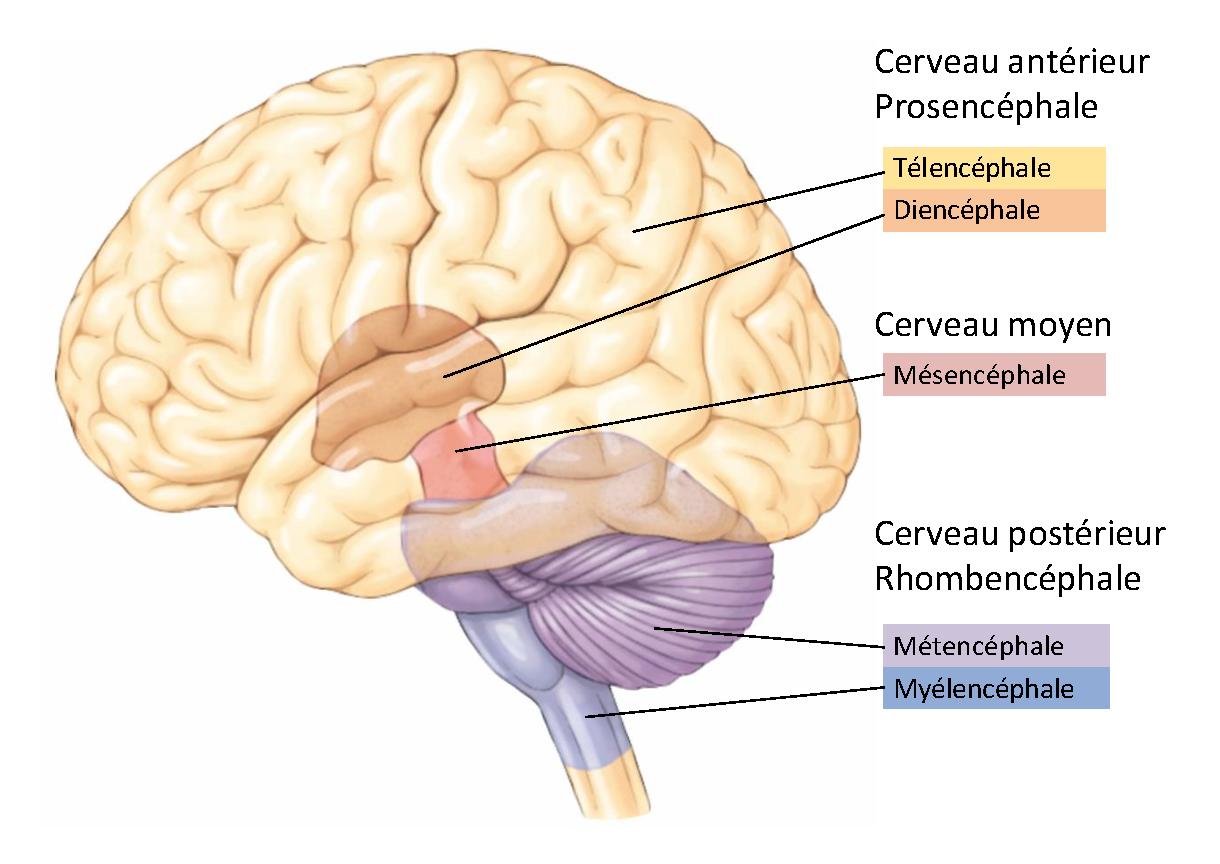
\includegraphics[width=0.5\textwidth]{Figures/1_cerveau.pdf}
	\caption{Division tripartite du cerveau humain : cerveau postérieur, cerveau moyen et cerveau antérieur.}
	\label{fig:cerveau}
\end{figure}

Le cerveau postérieur, considéré schématiquement comme le plus ancien dans la phylogenèse et le plus précoce dans l'embryogenèse, se divise en \emph{myélencéphale} et \emph{métencéphale}. 
Le myélencéphale assure la régulation des fonctions vitales, telles que la respiration, la pression artérielle, le rythme cardiaque et la digestion. 
Le métencéphale contient le pons et le cervelet. 
Le pons relie le tronc cérébral aux autres structures cérébrales et participe au contrôle de certains comportements et réflexes, et à la régulation des cycles veille–sommeil.
Le cervelet participe à l’ajustement en temps réel des actions, en comparant en permanence les commandes motrices émises avec leurs conséquences sensorielles effectives.
Il contribue à la prédiction de l’évolution future de la position du corps et des objets en mouvement à partir des informations sensorielles et motrices. 
Mikael Paulin parle d'un véritable \an{tracking system} :

\begin{quote}
	\an{The cerebellum may be better characterised as a tracking system, with an important role in control and coordination of movements which arises because of an animal's need to track moving objects, to track its own movements, and to analyse the sensory consequences of movements in order to control movements.}
	\cite{paulin_role_1993}
\end{quote}

Le cerveau moyen participe à l’intégration et au traitement précoce des informations sensorielles de toutes origines : somatosensorielles, visuelles, auditives, et même, chez certaines espèces, d’autres modalités telles que l’électrolocation. 
Il contient le \emph{tectum} (colliculus supérieur et inférieur chez les mammifères), qui joue un rôle majeur dans la localisation spatiale égocentrique de ces signaux sensoriels. 
Le tectum effectue une intégration multimodale fondée sur des coïncidences spatiales et temporelles.
Il est organisé en couches formant des cartes spatiales égocentrées et alignées pour chaque modalité sensorielle, de sorte qu’un même point de l’espace est représenté de manière congruente pour toutes les modalités. 
Des interconnections entre les cartes sensorielles et les cartes motrices permettent une coordination sensorimotrice rapide \cite{isa_tectumsuperior_2021}.

Le cerveau antérieur, dont le développement est le plus récent dans la phylogenèse et le plus tardif dans l'ontogenèse, est formé du \emph{diencéphale} et du \emph{télencéphale}. 
Le diencéphale contient le thalamus et l'hypothalamus qui sont impliqués dans la régulation des états internes en intégrant les émotions, les motivations et les désirs.
Le télencéphale contient les ganglions de la base, l'amygdale, l’hippocampe et le cortex, qui connecte les expériences spatio-temporelles et les motivations aux fonctions dites de haut niveau telles que l'interprétation d'information, la prise de décision, la navigation, la mise en \oe uvre d'activités complexes, la mémorisation, l'apprentissage, et, chez l'humain, le langage et le raisonnement abstrait.

Il me semble important de retenir que les aspects physiologiques et interoceptifs traversent tous les niveaux de ce découpage tripartite, du plus ancien au plus récent. 
En particulier la dimension émotionnelle et la dimension de la corporéité spatio-temporelle sont étroitement connectées à chaque niveau ce qui les place au centre de l'activité cérébrale.
Je développe davantage ces deux dimensions dans les sections suivantes.
%Il me semble important de retenir qu'il y a deux dimensions de l'activité cérébrale qui se projettent à tous les niveaux de ce découpage tripartite, du plus ancien aux plus récent: la dimension affective et la dimension de la spatio-temporelle. 


\subsection{Émotions}

\noindent
Les émotions occupent une place centrale dans la vie mentale en la rattachant à la condition vivante du corps. 
De nombreux auteurs soulignent l'importance de leur inscription corporelle, notamment Antonio Damasio dans sa théorie des marqueurs somatiques \cite{damasio_descartes_1994}. 
Elles constituent, presque par définition, un élément fondamental de la motivation et de la prise de décision. 
Elles participent à l’orientation de l’attention, à l’évaluation de l’environnement et à la sélection des comportements.
%Les émotions occupent une place centrale dans la vie mentale et constituent, presque par définition, un élément fondamental de la motivation et de la prise de décision. 

De nombreux modèles théoriques des émotions ont été proposés. 
Dès le XIX\ieme{} siècle, Darwin identifie et décrit une trentaine d’émotions dans son ouvrage \og \emph{The Expression of the Emotions in Man and Animals} \fg{}, qu’il regroupe en sept catégories principales \cite{darwin_expression_1872}. 
Depuis, la question du nombre et de la nature des émotions fondamentales reste débattue mais un consensus relatif semble se former autour d'un nombre d'émotions de base compris entre cinq et dix.

Max Talanov et son équipe a proposé une revue des différents modèles d'émotion utilisés en robotique qui les ont conduits à utiliser le \emph{cube des émotions} de Lövheim \cite{lovheim_new_2012}. 
Ce modèle propose une représentation continue de l’état émotionnel fondée sur le taux de concentration relatif de trois neuromodulateurs : la dopamine (DA), la sérotonine (5-HT) et la noradrénaline (NE), comme illustré en Figure~\ref{fig:emotions}.

\begin{figure}[th]
	\centering
	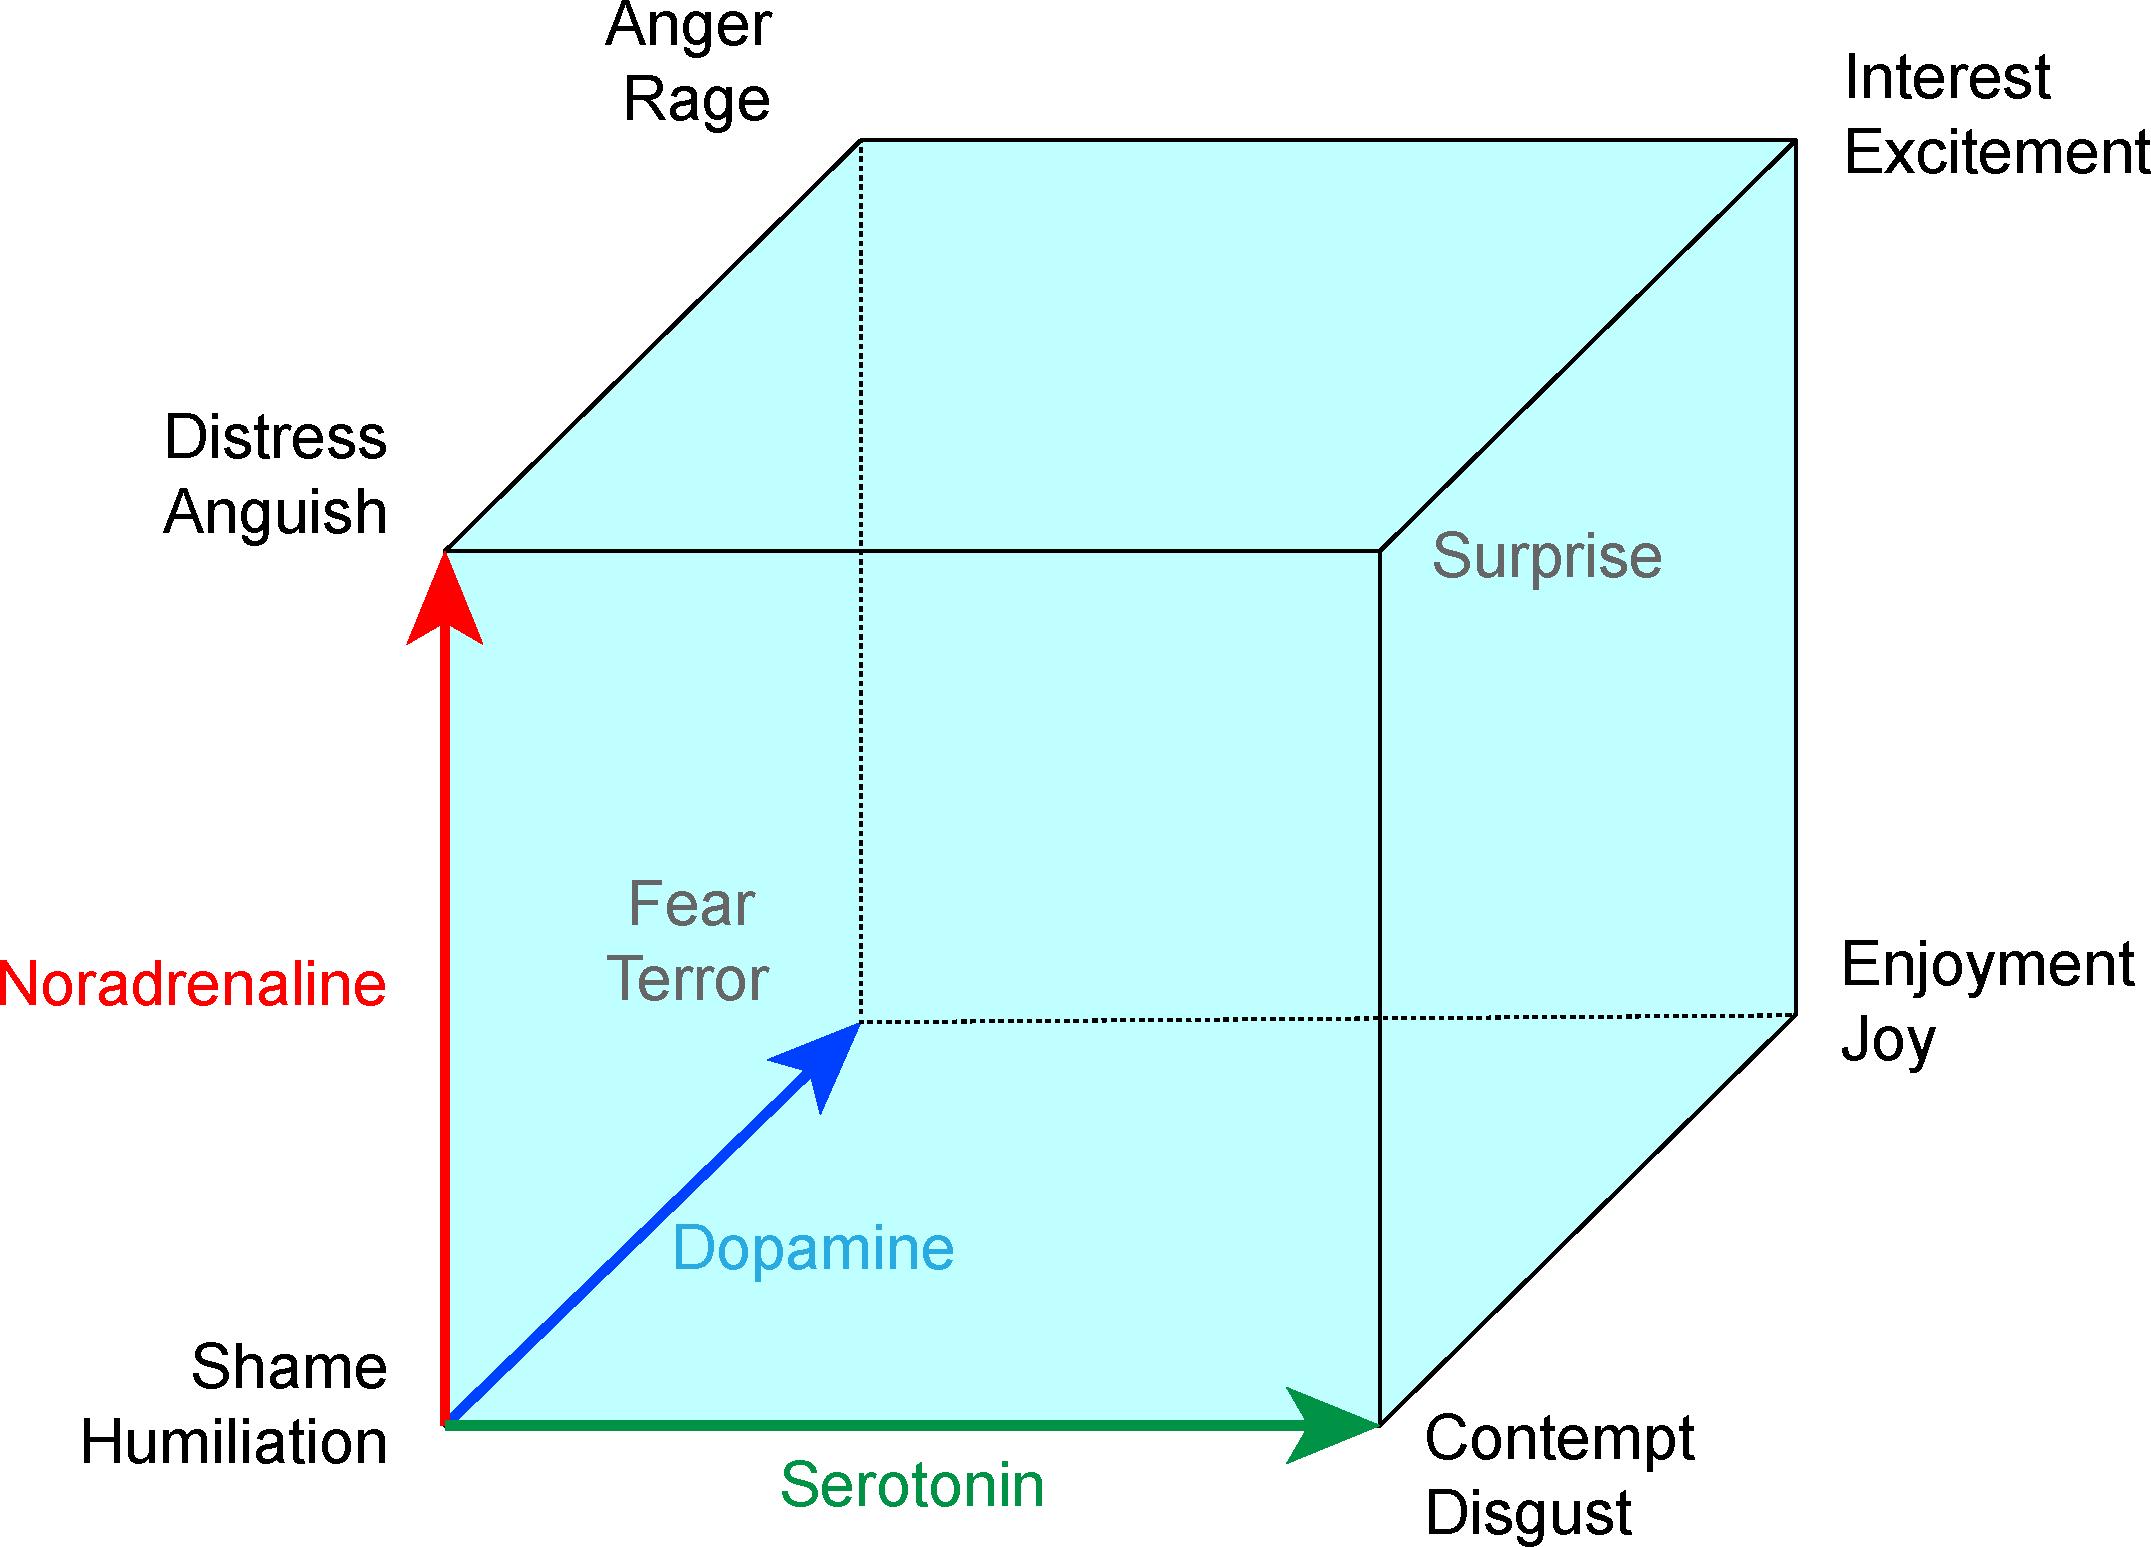
\includegraphics[width=0.5\linewidth]{Figures/1_Lovheim_cube_of_emotion.pdf}
	\caption{Le cube des émotions de Lövheim \cite[Fig.~1]{lovheim_new_2012}, délimité par les valeurs minimales et maximales de la sérotonine (5-HT), dopamine (DA) et noradrénaline (NE). 
		La sérotonine est associée à la confiance en soi, la dopamine aux situations marquantes produisant un renforcement de la mémoire, et la noradrénaline à la vigilance.
		L'état émotionnel neutre est représenté par le point central du cube.}
	\label{fig:emotions}
\end{figure}

Lövheim indique qu'il existe plusieurs dizaines de types de neurotransmetteurs impliqués dans les émotions et que le choix de ces trois principaux constitue un premier ordre d'approximation de toute la palette des émotions possibles.  
Il explique que ces trois neurotransmetteurs sont très anciens dans l'échelle phylogénétique et sont présents chez des animaux allant des nématodes au vertébrés. 
Chez l'homme, il sont produits par des petits groupes de neurones situés dans la partie haute du tronc cérébral et qui projettent leurs axones et diffusent ces neurotransmetteurs à travers tout le cortex. 
L'amygdale, située dans le telencéphale, joue un rôle crucial dans le contrôle de leur production et leur régulation.

Bien que chacun de ces trois neurotransmetteurs soit associé à une dimension affective dominante, Lövheim insiste sur l’existence probable d’interactions dynamiques complexes entre eux.
Il ne considère pas que les états émotionnels soient associé à des comportements spécifiques à chaque situation mais au contraire qu'ils ont un effet général tout en présentant une dynamique suffisamment rapide pour permettre une adaptation de survie efficace aux changements de l’environnement. 

La sérotonine renvoie à des aspects tels que la confiance en soi (\an{confidence}) et l'attitude posée.
Les quatre sommets du cube situés du coté de la sérotonine élevée correspondent à des situations propices à l'apprentissage et possiblement ludiques, y compris le sommet \an{Contempt/Disgust} (mépris, dégout) qui est à prendre dans le sens positif d'un refus calme et d'une capacité à dire \og non \fg. 
Les états de sérotonine faible sont associés à des situations de découragement ou de détresse. 

La dopamine est associée à la recherche de récompenses positives et à l'évitement de punitions.
Les quatre sommets du cube situés du coté de la dopamine élevée correspondent à des situations marquantes liées à un renforcement de la mémoire d'expériences positives ou négatives.
Au contraire, les sommets du coté de la dopamine faible correspondent à des expériences fades, y compris la \emph{surprise} qui est à comprendre ici en tant qu'elle n'est encore pas qualifiée. 
Elle pourra être suivie rapidement d'autres émotions selon qu'elle est bonne ou mauvaise.

La noradrénaline est liée au niveau de vigilance. 
Les sommets situés du coté de la noradrénaline élevée sont liés à un fort engagement: \an{anger/rage} peut être lié à des comportements de fuite ou de combat, alors que \an{Distress/Anguish} (détresse, angoisse) correspond à un état de fébrilité ou de tourment.
Ceux situés du coté de la noradrénaline faible sont liés à des états de sidération comme \an{Fear/Terror} ou de béatitude comme \an{Enjoyment/Joy}. 

Talanov montre que l’intégration du modèle émotionnel de Lövheim permet de concevoir des robots dont les actions ne sont pas uniquement dictées par des objectifs externes ou des règles prédéfinies, mais émergent également de dynamiques motivationnelles internes. 
Cette approche favorise la diversité et la variabilité des comportements, les rendant plus naturels et plus engageants pour les humains en interaction avec le robot.

Le modèle de Lövheim suggère donc de représenter l'état émotionnel d'un robot sous forme de trois variables continues indépendantes qui peuvent moduler la sélection des comportements. 
Il ne s'agit par se prétendre que le robot éprouverait des émotions ni même qu'il serait \og doté d'un système émotionnel \fg, mais plutot d'examiner l'hypothèse que ce modèle permettrait de créer un robot qui mimerait les émotions et permettre des apprentissages ouverts.
La sérotonine pourrait promouvoir des comportements de résolution de problème et d'expérimentation afin de tester ou d'affiner un modèle interne du monde. 
La dopamine serait liée à des apprentissages par renforcement positif ou négatif, par exemple à l'occasion d'exploration de nouvelles zones de l'environnement. 
La noradrénaline pourrait favoriser des comportements d'interaction et de collecte d'information liés à une focalisation de l'attention sans nécessairement être liés à l'apprentissage à long terme. 


\subsection{Représentations spatio-temporelles}

\noindent
György Buzsáki et Edvard Moser ont avancé l’hypothèse selon laquelle les mécanismes neuronaux sous-jacents à la navigation dans l’espace physique et l'espace mental reposeraient sur des principes communs \cite{buzsaki_memory_2013}.
Les représentations spatio-temporelles pourraient ainsi servir de fondement à la cognition abstraite. 
Selon eux, ces représentations sont intimement liées à l'activité du corps et au contrôle du mouvement. 
Les rythmes des boucles moteur-sensorielles seraient à la base du référentiel spatial et temporel.  
Il suggèrent que le cerveau s'appuierait sur ces capacités de calcul spatio-temporel héritées de l'évolution phylogénétique, et précoces sur le plan du développement ontogénique, pour naviguer dans des espaces conceptuels abstraits.  

%\begin{quote}
%	\og \an{the neuronal algorithms underlying navigation in real and mental space are fundamentally the same} \fg
%	 \cite[p.~130]{buzsaki_memory_2013}.
%\end{quote}

Comme évoqué à la section \ref{sec:anatomie}, des capacités de calcul spatio-temporel sont présentes à tous les niveau du découpage tripartite du cerveau. 
Dans le télencéphale, le complexe entorhinal-hippocampal joue un rôle central dans l'organisation des activités spatio-temporelles complexes. 
Il contient un ensemble de neurones spatialement modulés, dont la découverte a conduit au prix Nobel de médecine en 2014 de John O'Keefe et Moser. 

Hideyoshi Igata et ses coauteurs ont montré que des neurones de l'hippocampe pouvaient rejouer des séquences en ordre inversé afin de reconstruire les positions ayant conduit à une récompense. 
Ils ont même observé que l’hippocampe pouvait rejouer des trajectoires optimisées qui n’avaient pas été directement explorées par l’animal \cite{igata_prioritized_2021}. 
Stéphanie Theves a montré que l'hippocampe code des distances pertinentes dans un espace conceptuels défini par des caractéristiques d'objets, suggérant l'existence d'une cartographie cognitive des concepts  \cite{theves_hippocampus_2019}. 
Eric Knudsen a montré que des neurones hippocampiques chez le primate peuvent former des \og gradients de valeur \fg\ le long d’un continuum abstrait de récompense, constituant une carte cognitive d’un espace de valeur motivationnelle (\an{value place field}) \cite{knudsen_hippocampal_2021}.


La plupart des auteurs soulignent toutefois l'ampleur de ce qu'ils nous restent encore à comprendre concernant la manière dont le cerveau gère l'espace et le temps. 
Dans leur article \og \an{The representation of space in the brain} \fg, Roddy Grieves et Kate Jeffery tentent une synthèse des études actuelles sur cette question \cite{grieves_representation_2017}. 
Je reproduis l'une de leurs figures en Figure \ref{fig:space} pour donner un aperçu général de la complexité des ces mécanismes. 

\begin{figure}[t]
	\centering
	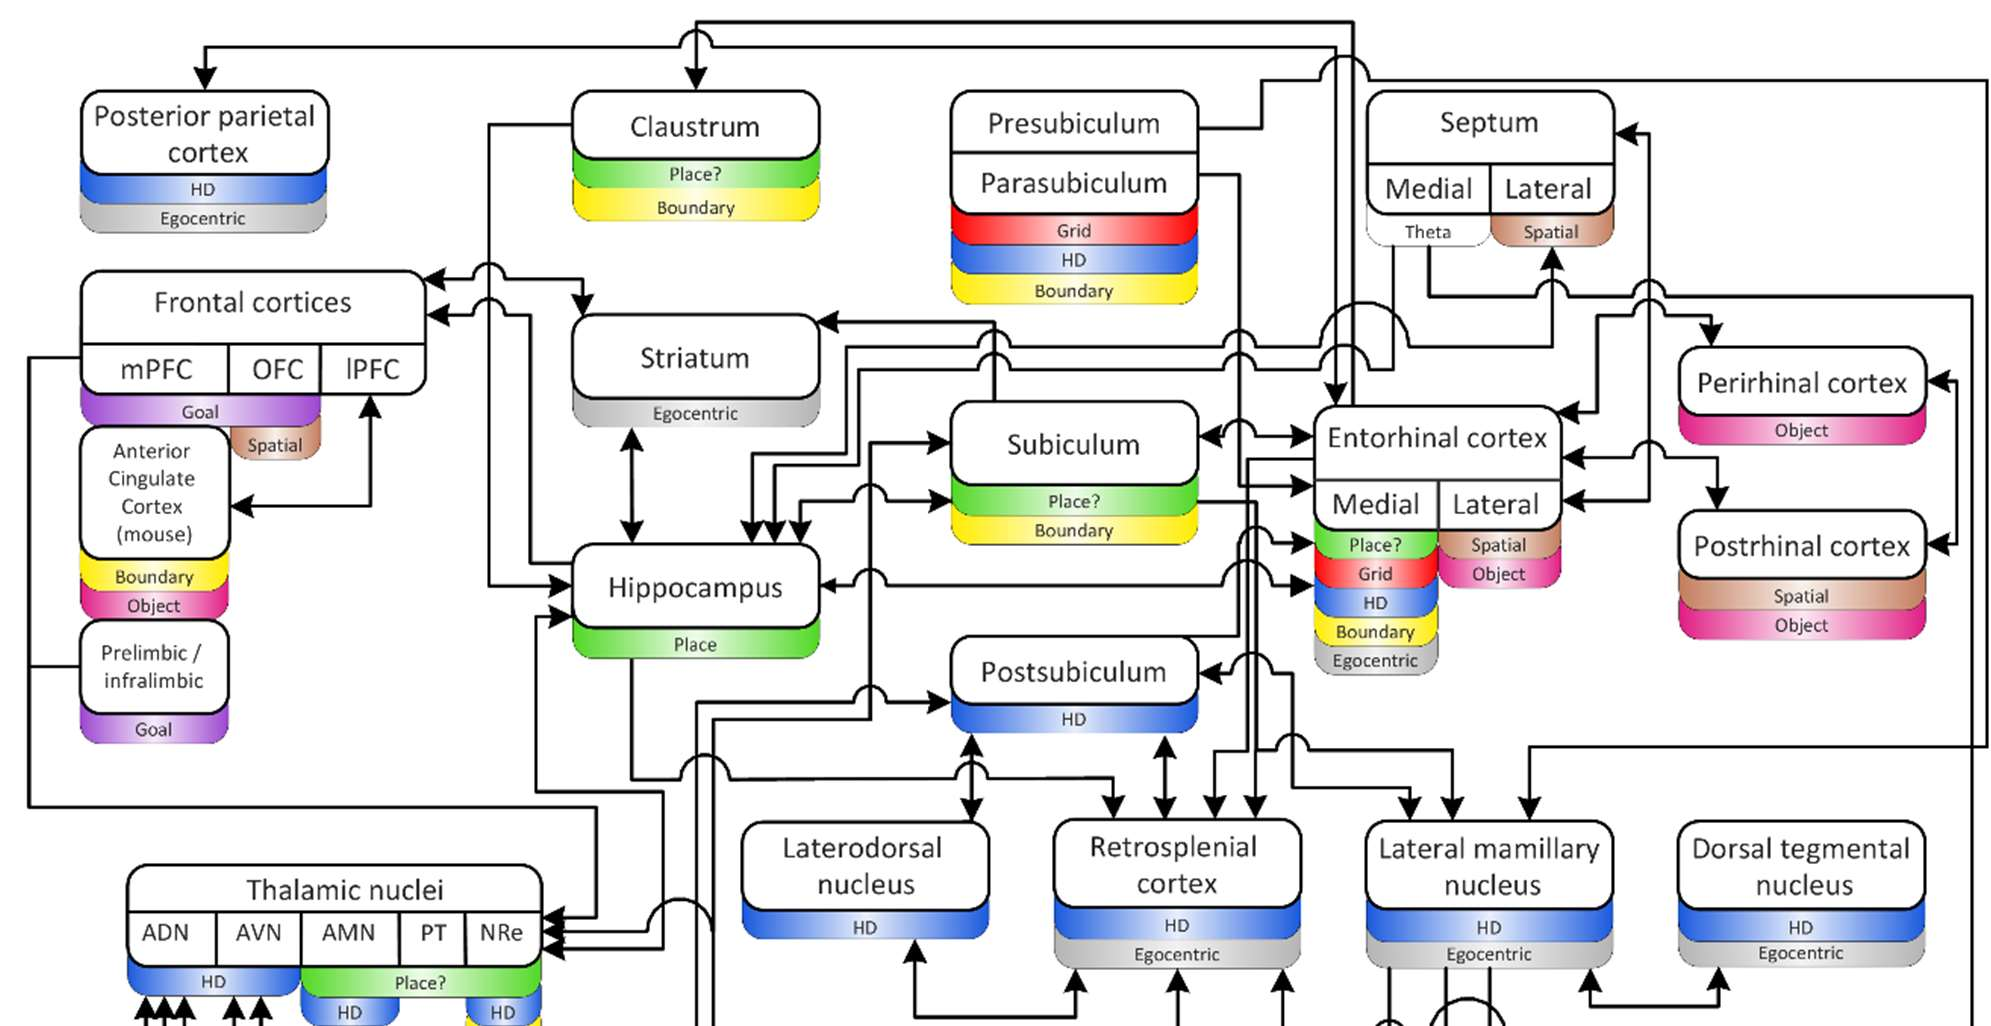
\includegraphics[width=0.7\linewidth]{Figures/1_space1.png}\\[-0.1em]
	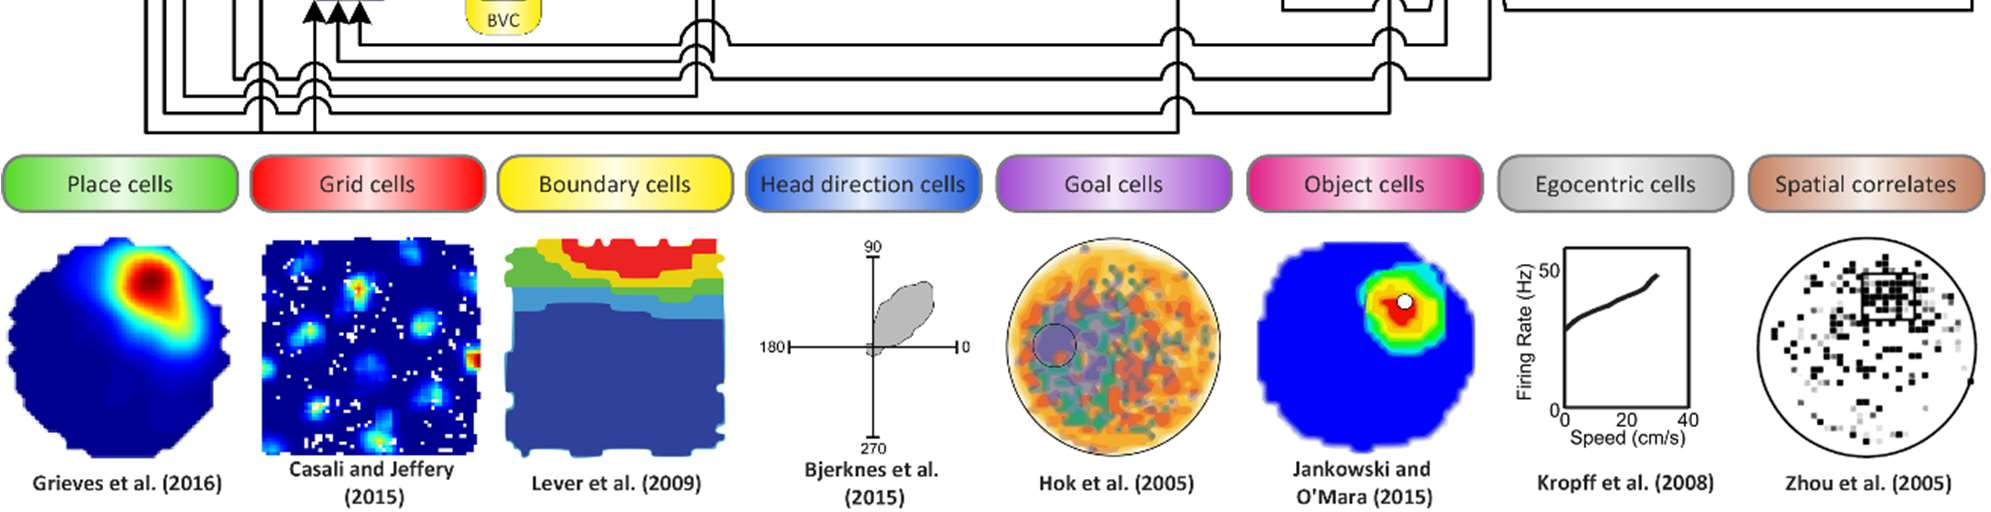
\includegraphics[width=0.7\linewidth]{Figures/1_space2.png}
	\caption{Synthèse des études sur la représentation de l'espace dans le cerveau par Grieves et Jeffery  \cite[Fig.~8]{grieves_representation_2017}. 
	}
	\label{fig:space}
\end{figure}

Grieves et Jeffery énumèrent de nombreux types de neurones impliquées dans la représentation spatio-temporelles en soulignant qu'on peut encore s'attendre à d'autres découvertes.
Les \an{place cells} représentent un réseau de positions identifiées dans un environnement donné, certaines \an{place cells} spécifiques s’activant lorsque l’animal occupe une position particulière dans l'environnement. 
Leurs champs d’activation émergent de l’intégration d’informations plus élémentaires telles que la direction, les frontières de l’environnement et les signaux de mouvement permettant de se rendre d'une place à l'autre. 
Lorsque l'animal change d'environnement, la population de \an{place cells} est reconfigurée (\an{remapped}) pour contribuer à la navigation dans ce nouvel environnement.
La façon dont cette reconfiguration s'opère nous est encore largement inconnue sachant que le cerveau ne voit pas directement le monde. 

Les \an{head-direction cells} encodent l’orientation de la tête par rapport à un repère allocentrique. 
Leur activité dépend à la fois d’indices sensoriels et de mécanismes d’intégration du mouvement. 
Les \an{grid cells} présentent une organisation spatiale périodique formant un pavage triangulaire. 
Elles seraient impliquées dans l’intégration du trajet (\emph{path integration}) et fourniraient un système de mesure des distances.
%Elles pourraient contribuer à l’estimation de la distance à une cible.
Les \an{speed cells} codent la vitesse de déplacement.
Les \an{boundary cells} répondent quand l'animal rencontre une bordure de l'environnement dans une direction allocentrique spécifique. 

Grieves et Jeffery soulignent que l'hippocampe est connu pour être impliqué dans des processus qui vont au delà de la navigation spatiale, comme la mémoire épisodique et la discrimination d'objets. 
Il mentionnent les \an{object cells} qui répondent à la présence d'un objet à un emplacement particulier, ou à l'absence d'un objet attendu à un endroit. 
Ils rapportent également des études investiguant des populations de neurones codant l'espace au delà de la région entorhinal-hippocampal. Certaines de ces études portent sur les \an{goal cells} dans le cortex préfrontal médian.
D'autres sur le codage de l’espace en relation avec l’action. 
Par exemple, certains neurones du striatum s’activent préférentiellement lorsqu'un mouvement spécifique est exécuté à un endroit particulier, permettant l’apprentissage d’actions, la formation d’habitudes et l’automatisation comportementale.
Des \an{conjunctive cells} encodent simultanément des caractéristiques spatiales et comportementales. 
Certaines ont été observées dans le cortex pariétal supérieur et dans le cortex rétrosplénial.


Ces résultats ont inspiré un certain nombre d'études en robotique portant sur la navigation bio-inspirée, 
par exemple celle de mon ancien doctorant Simon Gay \cite{gay_towards_2021}.
A ma connaissance, cependant, aucune simulation informatique ou robotique ne se rapproche pour l'instant du niveau de complexité décrit par Grieves et Jeffery.

Dans le domaine de l'IA, Jeff Hawkins a proposé la \an{Thousand Brains Theory} basée sur l'hypothèse que des mécanismes analogues aux \an{grid cells} seraient distribués au sein de nombreuses colonnes corticales  \cite{hawkins_framework_2019}. 
Selon lui, l’intelligence s'appuierait sur l’interaction de milliers de modèles locaux spatio-temporels capables d’apprendre la structure des objets et de l’environnement.
Ces neurones serviraient de base à  un système de coordonnées universel permettant d’organiser différents types de connaissances. 




\subsection{Socle de connaissances}
\label{sec:core}

\noindent
Certains auteurs ont étudié les systèmes de géométrie mentale sur le plan de l'éthologie et de la psychologie développementale. 
Ces études apportent un niveau d'analyse complémentaire au niveau neuro-anatomique présenté à la section précédente. 
Le récent livre de Stanslas Dehaene \og Le Rectangle de Lascaux: et homo sapiens inventa la géométrie \fg\ passe en revue ne nombreuses études mettant en évidence les prédispositions du cerveau humain à manipuler des représentations géométriques et temporelles \cite{dehaene_rectangle_2026}.  
Dans leur article \og \an{Core systems of geometry in animal minds} \fg, Elizabeth Spelke et Sang Ah Lee identifient plusieurs systèmes de géométrie fondamentaux qui seraient apparus au cours de l'évolution bien avant l'apparition de l'espèce humaine. 
Elles rapportent deux systèmes géométriques distincts: le système fondamental de navigation (\an{core navigation system}) et le système fondamentale d'analyse de formes (\an{core form analysis system}).  
Elles proposent l'hypothèse que ces deux systèmes fondamentaux donneraient lieu à des intuitions géométriques abstraites chez l'humain. 

Le \an{core navigation system} est spécialisé dans la représentation des distances absolues et l'identification des directions.
Il repose sur un mécanisme automatique et un mécanisme attentionnel de navigation. 
Le mécanisme automatique se baserait sur la forme des bordures de l'environnement tels que des surfaces verticales, alors que le mécanisme attentionnel utiliserait des points de repères (\an{landmarks}) visuels. 
Certaines études ont même tenté de déterminer ce qui comptait comme contour de l'environnement: des murs ou mêmes des légères marches sur le sol \cite{cheng_purely_1986}. 
Inversement, des lignes ou des contours dessinées sur le sol n'étaient pas prise en compte comme contour ni des colonnes espacées.  
 
%Ken Cheng a mis en évidence le système 1) chez des rats en montrant qu'ils utilisaient la forme des murs de l'enceinte dans laquelle ils étaient placés pour retrouver de la nourriture cachée .  En l'absence d'entrainement, ils n'utilisaient pas de points de repères tels que la couleur des murs ou des marques sur les murs. 

Le \an{core form analysis system} permet à des animaux, allant des insectes aux humains, de  reconnaitre des formes visuellement. 
Se système se base sur les relations relatives entre longueurs et sur les angles. Il se caractérise par une invariance d'échelle et une invariance de sens, c'est à dire qu'il est relativement insensible aux différences d'échelle et aux retournement en miroir.
Spelke souligne que les deux systèmes apparaissent donc pratiquement complémentaire: le système de navigation capture des distances absolue et le sens mais pas les longueurs relatives ni les angles, le système de reconnaissance de forme fait l'inverse. 

Au delà du système de géométrie, certains auteurs se sont intéressés à un système de physique intuitive mentale. 
Joshua Tenenbaum  et son équipe \cite{ullman_mind_2017} a proposé l'idée de \an{game engine in the head} (GEITH), ou moteur de jeu mental comme une métaphore pour décrire la façon dont l’esprit humain raisonnerait sur le monde physique.
L’hypothèse est que le cerveau contient un \og moteur de physique intuitif \fg\ analogue aux moteurs physiques utilisés dans les jeux vidéo : 
un système interne qui simule approximativement la dynamique des objets (chutes, collisions, empilements, écoulement de liquides, etc.) pour prédire leur trajectoire (Figure \ref{fig:geith}).

\begin{figure}[t]
	\centering
	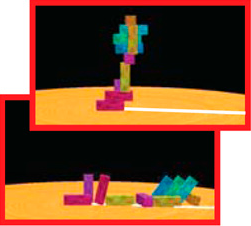
\includegraphics[height=0.3\linewidth]{Figures/1_geith.png}%
	\quad
	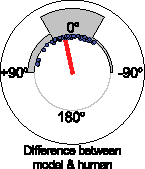
\includegraphics[height=0.3\linewidth]{Figures/1_geith.pdf}
	\caption{Expérimentation sur le \an{Game Engine In The Head} \cite[Fig.~3]{ullman_mind_2017}. 
		Gauche: l'expérimentateur demande aux sujets d'indiquer dans quelle direction ils estiment que la tour va tomber. 
		Droite: mesure de l'écart entre la prédiction du sujet et celle de l'ordinateur.
	}
	\label{fig:geith}
\end{figure}


Les \an{core knowledge} ne se limitent pas à la géométrie et à la physique. 
François Chollet \cite{chollet_measure_2019} a listé quatre savoirs fondamentaux que la plupart des agents  intelligent naturels auraient hérités de l'évolution phylogénétique : 
\begin{itemize}[label=\scalebox{.85}{$\diamond$}]
	\item Géométrie élémentaire, spatialisation: reconnaitre et manipuler des formes simples (lignes, rectangles, triangules, cercles). Différentier les formes même après des transformations (rotation, translation, symétrie, déformation). Détecter les positions et distances. 
	\item Objets et leur persistance: Les objets existent de manière continue ; ils ne peuvent pas apparaître ou disparaître sans raison; ils peuvent interagir selon les circonstances.
	\item Nombres et comptage: il est possible de compter des petits nombres d'objets ou propriétés, et former des groupes dénombrés.
	\item Agentivité : certains objets peuvent être identifiés comme \og agents \fg poursuivant une intention ou un but. On distingue les objets animés et inanimés.
\end{itemize}

Ces études sur le \an{core knowledge in the mind} nous apportent un éclairage sur la répartition entre l'inné et l'acquis dans le système cognitif animal et humain. 
Cet éclairage peut guider la conception de nos robots développementaux en aidant à déterminer quelles structures ou contraintes seront  \og codées en dur \fg\ et lesquelles seront laissées à l'apprentissage au cours d'interaction avec l'environnement. 


\subsection{Comportements instinctifs}

\noindent
De nombreux animaux manifestent des comportements propres à leur espèce qui semblent essentiels à leur survie. 
Les exemples sont multiple: construction de toiles chez les araignées, poursuite d'objets en mouvements chez les chien et les chats, ou encore migration chez diverses espèces terrestres, volantes, ou aquatiques. 
La manière dont ces comportements se transmettent d'une génération à l'autre, et la part de l'inné et de l'acquis, fait l'objet de nombreuses interrogations en éthologie. 
Selon Blumberg, par exempe : 


\begin{quote}
	\an{Various animals are said to possess a survival instinct, migratory instinct, herding instinct, maternal instinct, or language instinct. But a closer look reveals that these and other “instincts” are not satisfactorily described as inborn, pre-programmed, hardwired, or genetically determined.
		Rather, [...] species-typical behaviors develop, and they do so in every individual under the guidance of species-typical experiences occurring within reliable ecological contexts.
	}
	\cite[p.~1]{blumberg_development_2017}	
\end{quote}

Blumberg précise que la nature développementale des comportements instinctifs ne signifie pas que tous les comportements instinctifs soient également malléables. 
Au contraire, ils s'inscrivent sur un continuum allant des plus rigides aux plus flexibles. 
Chez les mammifères, par exemple, l'orientation du nouveau-né vers la source de lait dès la naissance apparait comme un comportement rigide et vital. 
Les signaux olfactifs y jouent un rôle central, mais ce comportement implique déjà un apprentissage sensorimoteur, combinaison également des indices tactiles, et parfois thermiques, comme l'ont montré Charlotte Hym et ses coauteurs chez l'humain  \cite{hym_newborn_2021}, ainsi que Jeffrey Alberts et April Ronca chez d'autres mammifères \cite{alberts_experience_2012}. 

Les comportements dits instinctifs ne sont donc pas des programmes codés dans les gènes qui seraient exécutés tels-quels dès la naissance. 
Ils résultent plutôt de prédispositions innées et de tendances qui orientent l'apprentissage dans des contextes et environnements spécifiques, lesquels jouent un rôle déterminant dans leur expression. 
Certaines de ces dispositions initiales sont communes aux humains et aux autres mammifères. 


A ma connaissance, l’apprentissage développemental précoce de comportements instinctifs fondé sur des préférences innées ne constitue pas, à ce jour, un domaine de recherche explicitement identifié en intelligence artificielle développementale. 
Cette problématique représente ainsi une contribution originale de mon travail.

\subsection{Psychologie développementale}

\noindent
Parallèlement à l'épistémologie génétique évoquée en Section \ref{sec:epistemologie_genetique}, Piaget a fondé le champ de la \emph{psychologie développementale}. 
Au-delà des dimensions théoriques de la construction du sujet connaissant, la psychologie développementale tente de décrire et comprendre le cheminement chronologique qui conduit l'esprit humain depuis l'état du nouveau-né jusqu'à celui de l'âge adulte.
Elle offre un pendant expérimental à l'épistémologie génétique, en s'appuyant sur des observations, permettant l'expérimentation, et proposant des applications. 
Dans son ouvrage \emph{Pour comprendre Jean Piagiet} \cite{dolle_pour_1997}, Jean-Marie Dolle synthétise ainsi les stades chronologiques du développement cognitif de l'être humain :

\begin{enumerate}[itemsep=0pt, parsep=0pt, partopsep=0pt]
	\item L'intelligence sensorimotrice
	\begin{enumerate}[itemsep=0pt, topsep=0pt, parsep=0pt, partopsep=0pt]
		\item Développement des structures sensorimotrices
		\begin{itemize}[label=\scalebox{.85}{$\diamond$}, itemsep=0pt, topsep=0pt, parsep=0pt, partopsep=0pt]
			\item Maitriser son propre dispositif
		\end{itemize}
		\item La construction du réel
		\begin{itemize}[label=\scalebox{.85}{$\diamond$}, itemsep=0pt, topsep=0pt, parsep=0pt, partopsep=0pt]
			\item La construction de l'objet permanent
			\item La construction de l'espace sensorimoteur
			\item La construction de la causalité
			\item La construction du temps
		\end{itemize} 
	\end{enumerate} 
	\item La genèse des opérations concrètes
	\begin{enumerate}[itemsep=0pt, topsep=0pt, parsep=0pt, partopsep=0pt]
		\item Intelligence représentative
		\item L'intelligence symbolique
		\item La mise en place des structures des opérations concrètes
		\item L'espace
	\end{enumerate} 
	\item L'intelligence opératoire formelle 
\end{enumerate}

Piaget ne conçoit pas ces étapes comme des phases nettement délimitées mais plutôt comme des repères jalonnant une trajectoire développementale continue. 
Dans un premier temps, l'enfant acquière une intelligence sensorimotrice (étape 1) qui lui permet de maitriser son appareil perceptif et moteur afin de se déplacer et interagir efficacement avec les éléments de son environnement en construisant des chaines causales. 
Il développe ensuite un système symbolique sur la base des objets concrets (étape 2), avant d'accéder à une intelligence plus générale basée sur le langage et le raisonnement logico-mathématique (étape 3). 

Depuis ce premier cadre posé par Piaget, la psychologie développementale s'est considérablement enrichie, remettant en question la temporalité et la chronologie des stades de développement. 
Philippe Rochat et Tricia Striano, par exemple, ont conçu une expérience montrant que des nourrissons âgés de seulement deux mois étaient déjà capables de se fixer des objectifs.
Ils pouvaient mobiliser certains comportements issus de leur répertoire inné et les adapter de manière circonstanciée pour atteindre ces objectifs.
Leur expérience offrait la possibilité aux nourrissons de modifier leur rythme de succion pour obtenir certains résultats sensoriels tels qu'entendre la voix de leur mère, se voir présenter certaines images, ou encore obtenir leur lait préféré \cite{rochat_emerging_1999}. %de l'ouvrage \an{Oxford handbook of human action} 
Le chapitre \an{The origins and sources of action} de Bernhard Hommel et Birgit Elsner  \cite{hommel_acquisition_2009} passe en revue de nombreuses expériences mettant en évidence l'habileté d'enfants âgés de deux à quatre mois à acquérir une maitrise des relations action-effet.
Ces enfants s'engageant spontanément dans des activités ludiques consistant à identifier simultanément des buts possibles et les opérations permettant de les atteindre.
Ils répètent ensuite ces activités en se perfectionnant et en manifestent de la joie en cas de réussite et de la déception en cas d'échec.  

D'autres études ont montré qu'une valence affective était généralement apprise en association avec les schèmes sensorimoteurs. 
Tom Becker et ses coauteurs \cite{beckers_automatic_2002}, par exemple, ont mis cette association en évidence en mesurant des temps de réponse plus courts en cas de congruence des valences affectives. 
Des sujets adultes étaient entrainés à  répondre à un choix binaire de catégorie de mots affectivement neutres en pressant des boutons. 
L'une des réponses provoquait une légère décharge électrique.
Dans la phase de test, les sujets effectuaient la même tâche, mais avec des mots à valence affective positive ou négative. 
L'expérience a montré que les mots positifs étaient traités plus rapidement quand la réponse n'induisait pas de choc, et inversement pour les mots négatifs. 
En se référant à la \an{Theory of Event Coding (TEC)} de Hommel \cite{hommel_theory_2001}, Becker conclut que les sujets encodent des événements unitaires qui regroupent les informations sensorielles, motrices, et de valence affective. 

%La psychologie développementale de Piaget a inspiré le champ de l'intelligence artificielle développementale, comme nous le verrons dans les chapitres suivants. 
La temporalité et la chronologie des stades d'apprentissage identifiés par Piaget ont été contestés, mais le principe d'un continuum d'apprentissage ininterrompu, ancré sur l'expérience sensorimotrice, au cours duquel chaque apprentissage successif s'appuie sur le précédent reste largement accepté. 
Cette trajectoire continue a été illustré par les chercheurs en IA développementale Frank Guerin et Daniel McKenzie par la Figure \ref{fig:guerin}. 
Cette conception invite à ne pas \og prendre de raccourcis \fg\ en tentant de répliquer des stades d'apprentissages avancés qui ne seraient pas ancrés dans des stades antérieurs. 
L'ancrage sensorimoteur risquerait alors d'être rompu.
Retenons aussi que l'énergie motivationnelle endogène de l'enfant joue un rôle crucial.
Elle peut passer par une valence affective associée aux schèmes sensorimoteurs. 

\begin{figure}[t]
	\centering
	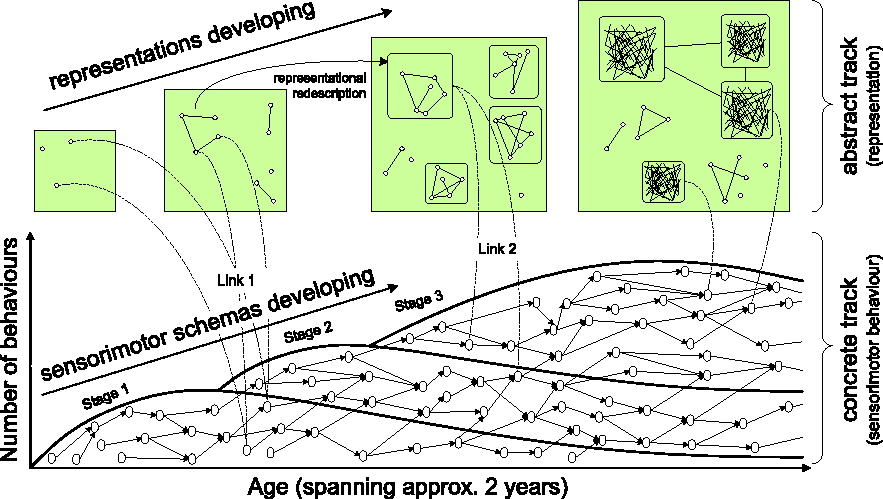
\includegraphics[width=0.7\linewidth]{Figures/1_guerin.pdf}
	\caption{Diagramme conceptuel du développement de l'enfant \cite[Fig.~1]{guerin_piagetian_2008}.
		Bas (\an{concrete track}): graphe de schèmes sensorimoteurs construit au cours du temps.
		Les n\oe uds sont des schèmes et les arcs sont des relations de dépendances entre schèmes. 
		Haut (\an{abstract track}): représentations des objets par réseaux de schémas qui décrivent les interactions que ces objets permettent.
	}
	\label{fig:guerin}
\end{figure}


% Hommel soulignent que, bien que les nouveaux-nés disposent déjà de capacités motrices et sensorielles, il est généralement admis qu'ils ne sont pas encore en mesure d'effectuer des actions intentionnelles \cite{hommel_acquisition_2009}. 
%Ils peuvent mouvoir leur corps et percevoir des événements sensoriels, y compris des réactions (\an{feedbacks}) résultants de leurs mouvements. 
%Les conséquences de leurs actions, qu'elles soient distales (visuelles ou auditives) ou proximales (tactiles, proprioceptives) sont enregistrées dès la naissance. 
%Les auteurs posent la question centrale : comment passons-nous de l'état de nouveau-né agité et réceptif à celui d'agent intentionnel ? 
%Hommel propose un modèle un deux étapes de l'acquisition d'actions volontaires : l'étape 1 consiste en l'apprentissage des contingences être les mouvements et les effets, et l'étape 2 consiste à se fixer des objectifs et utiliser cette connaissance pour les atteindre.   
%Certaines expériences montrent que le cortex premoteur pourrait intégrer les actions avec leurs conséquences attendues sous forme d'une sorte de \an{pragmatic body map} \cite{schubotz_functional_2001}. 








\section{Mesurer l'intelligence}

\noindent
Pour clore cette vue d'ensemble de la notion d'intelligence je dois aborder les méthodes permettant de l'évaluer et de la quantifier.
Legg et Hutter \cite{legg_universal_2007} proposent une synthèse des principales techniques de mesure de l'intelligence naturelle afin d'en dégager des pistes pour établir des \an{benchmark} d'évaluation de l'intelligence artificielle. 

Ils introduisent d'abord une distinction entre les \emph{tests statiques} et les \emph{tests dynamiques}. 
Les tests statiques évaluent la capacité à résoudre un problème présenté en une seule fois. 
Ils mettent l'accent sur l'exploitation de connaissance et la mise en \oe uvre d'un raisonnement pour produire une réponse correcte à une question posée. 
%Ils ne mesurent pas directement la capacité à apprendre et à s'adapter au cours du temps. 
A l'inverse, les tests dynamique se déroulent pendant une certaine période de temps au cour de laquelle l'agent interagit avec l'environnement de test. 
Ils visent à mesurer la capacité de l'agent à mettre en \oe uvre une stratégie qui peut donner lieu à un apprentissage au cours du déroulé du test. 

Legg et Hutter introduisent ensuite une second distinction, cette fois entre les tests fondés sur une \emph{mesure objective} et ceux fondés sur un \emph{jugement humain}.
Les premiers mesurent la capacité de l'agent à produire des réponses attendues ou à atteindre des objectifs préalablement définis.
Dans ce cadre, les auteurs esquissent l'idée d'une \og mesure universelle de l'intelligence \fg\ définie comme la somme infinie des score normalisés obtenus dans l'ensemble des environnement possibles, pondérée par la complexité de chacun d'eux. 
Ils reconnaissent qu'une telle mesure n'est pas calculable en pratique mais la proposent comme un modèle conceptuel utile de ce qu'ils appellent une \an{mesure of universal intelligence}. 
% la somme infinie sur tous les environnements possibles dans lequel la reward est computable avec une somme bornée, de la mesure de la capacité à atteindre l'ojectif normalisée dans l'interval [0, 1] pondérée par de manière inversement proportionnelle à la complexité de l'environnement. 

Certains auteurs défendent la nécessité d'un jugement humain. 
Parmi eux, Alexei Samsonovich soutient que si la mesure de l'intelligence est formalisée à l'avance alors il est toujours possible de \og hacker \fg\ le test par un algorithme qui n'adresse pas les questions fondamentales de l'intelligence. 
Il cite John von Neumann qui avait déjà formulé cette difficulté:  \og \an{If you will tell me precisely what it is that a machine cannot do, then I can always make a machine that will do just that} \fg\  \cite[p.~105]{samsonovich_roadmap_2012}.
Dans \og \an{Beyond reward and punishment} \fg, David Deutsch argumente qu'un système varitablement intelligent doit être capable de faire quelque chose pour lequel il n'a pas été spécifiquement programmé, voire désobéir aux instructions de ses concepteurs \cite{deutsch_beyond_2019}.
Le célèbre test de Turing s’inscrit précisément dans cette idée d'un jugement humain, puisqu'il demande à des observateurs humains de juger la capacité d’une intelligence artificielle à imiter une intelligence naturelle.

La Figure \ref{fig:mesures} récapitule les quatre quadrants délimités par les deux distinctions proposées par Legg et Hutter. 
 

\begin{figure}[ht]
	\centering
	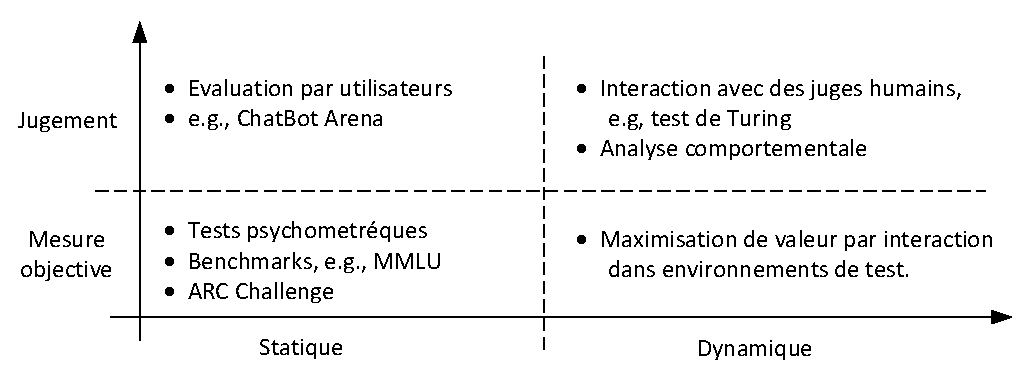
\includegraphics[width=0.8\textwidth]{Figures/1_mesures.pdf}
	\caption{Classification des modes d'évaluation de l'intelligence, inspirée par \cite{legg_universal_2007}.
	Horizontalement : réponses immédiates ou période d'interaction.
	Verticalement : mesures formalisées ou actes de jugement humain.}
	\label{fig:mesures}
\end{figure}

\subsection{Tests statiques}

\noindent
Les tests statiques ne sont pas pertinents pour évaluer les IA développementales car ils ne permettent pas de saisir les dynamiques d'apprentissage et d'adaptation au cours du temps. 
Ils s'appliquent principalement aux systèmes d'apprentissage supervisés et aux grands modèles d'IA générative. 
Je les passe en revue brièvement ici pour éclairer la classification de Legg et Hutter et parce que certains d'entre eux figurent parmi plus connus dans le paysage de l'IA actuelle.

Un premier exemple appartenant au quadrant \emph{statique} / \emph{objectif} est le \an{benchmark} \an{Measuring Massive Multitask Language Understanding} (MMLU) \cite{hendrycks_measuring_2021}. 
Il rassemble des questions couvrant un large champ académiques pour mesurer la solidité générale du raisonnement et la capacité à transférer les connaissances d'un domaines à l'autre.
Il présente l'inconvénient de nécessiter un jeu de questions-réponses fourni par des experts et inconnu du modèle, ce qui implique de le renouveler constamment.
Un autre inconvénient est qu'il ne distingue pas clairement ce qui relève de l'intelligence \og pure \fg\ et ce qui dépend de connaissances préalables, notamment en mathématiques ou en physique.

Le \an{Abstract Reasoning Challenge} (ARC) \cite{chollet_measure_2019} constitue un deuxième exemple de ce quadrant.
Il présente l'avantage de spécifier clairement les connaissances qu'il présuppose chez l'agent. 
Ce sont les \an{core knowledge} que j'ai listés en Section \ref{sec:core}: géométrie élémentaire, objets et persistance, nombre et comptage, agentivité.
%Pour éviter d'impliquer des savoirs scolaires et éducatifs, François Chollet propose le \an{Abstract Reasoning Challenge} (ARC) \cite{chollet_measure_2019}, un benchmark qui n'utiliser que les \an{core knowledge} listés en Section \ref{sec:core}.
%L'ARC Challenge constitue un second exemple intéressant du quadrant \emph{statique} / \emph{objectif}. 
Ce test s’inspire de la structure des tests psychotechniques et propose des problèmes de raisonnement abstrait fondés sur la détection de motifs et de transformations logiques. 
Il évalue ainsi la capacité d’un système à généraliser à partir d’exemples et à inférer des règles.
%La Fig. \ref{fig:ARC} montre un exemple mettant en jeu le \an{core knowledge} d'agentivité. Dans cet exemple, la règle à inférer pour passer de l'image de gauche à celle de droite est qu'un agent se déplace d'un point à un autre en tournant quand il arrive face à un carré vert. 

%\begin{figure}[ht]
%	\centering
%	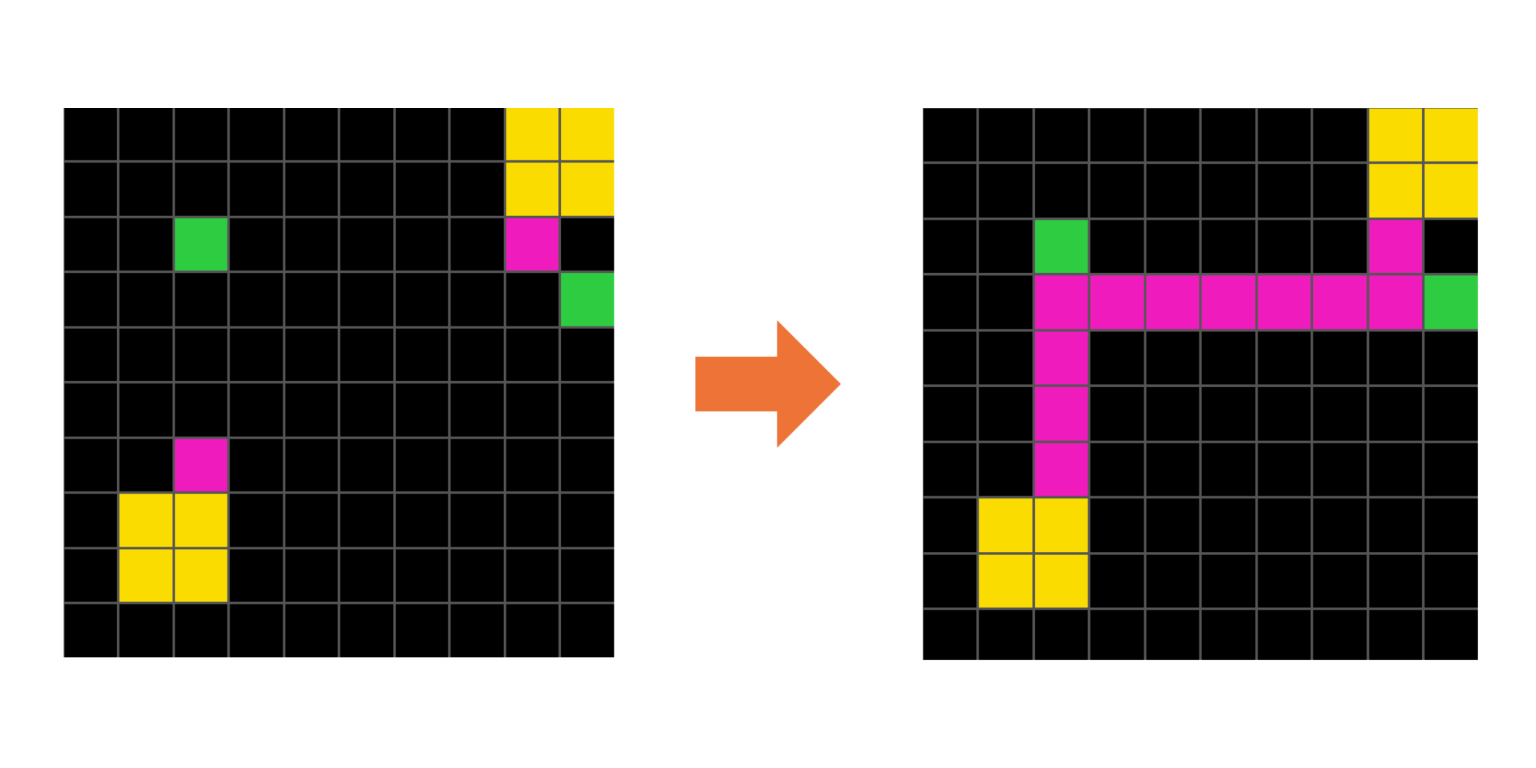
\includegraphics[width=0.6\textwidth]{Figures/1_ARC.png}
%	\caption{Exemple de problème du ARC Challenge impliquant le socle de connaissance d'agentivité. }
%	\label{fig:ARC}
%\end{figure}



Un exemple représentatif du quadrant \emph{statique} / \emph{jugement} est \an{Chatbot Arena} \cite{chiang_chatbot_2024}.
Ce \an{benchmark} évalue les LLMs en organisant des confrontations en aveugle opposant les modèles deux à deux.
Il produit un classement de type Elo sur la base d'un jugement humain \og crowdsourcé \fg, les utilisateurs proposant leurs propres prompts et sélectionnant la meilleure réponse sans connaitre les modèles en compétition. 

\subsection{Tests dynamiques}

\noindent
Les tests dynamiques concernent principalement les systèmes d'apprentissage non supervisés ainsi que les agents et robots autonomes. 
Le quadrant \emph{dynamique} / \emph{objectif} s'applique tout particulièrement à l'apprentissage par renforcement puisque celui-ci vise précisément à maximiser une valeur numérique (voir Section \ref{sec:rl}). 
Les jeux de plateau offrent des \an{benchmarks} emblématiques de ce quadrant. 
Un exemple marquant d'apprentissage par renforcement dans ce contexte est AlphaZero présenté dans \og \an{A general reinforcement learning algorithm that masters chess, shogi, and Go through self-play} \fg\ \cite{silver_general_2018}.

Le quandrant \emph{dynamique} / \emph{jugement} regroupe les évaluations de l'intelligence \an{open-ended} en milieu ouvert pour lesquels les objectifs finaux de l'agent ne sont pas explicitement fixés. 
Aucun test ne fait réellement figure de référence de ce quadrant auprès du grand public ou de la communauté scientifique.
L'idée du test de Turing illustre l’esprit de ce quadrant, mais n'a pas été mise en \oe uvre de manière convaincante. 
Des tentatives ont été menées, par exemple le \an{Loebner Prize}, lancé en 1990 et critiqué jusqu'à sa disparition en 2020, sans doute parce que l’objectif du test de Turing demeure hors de portée de l'IA actuelle \cite{powers_total_1998}.
En pratique, chaque équipe de recherche définit ses propres critères de jugement centrés sur les aspects de l'intelligence qu'elle souhaite explorer. 

En robotique, l'acte de jugement peut s'appuyer sur une analyse fine des comportements du robot. 
Alexander Maye et Andreas Engel démontrent par cette méthode que leur robot acquiert une maitrise des \og contingences sensorimotrice \fg\ (voir Section \ref{sec:SMC}).
Leur article \og \an{A discrete computational model of sensorimotor contingencies for  object perception and control of behavior} \fg\ \cite{maye_discrete_2011} présente un modèle de reconnaissance d'objets dans lequel les actions sont au c\oe ur du processus perceptif.
Leur analyse comportementale illustrée en Figure \ref{fig:maye} met en évidence les contingences sensorimotrices propres à un couplage robot-objet particulier, représentées sous la forme d’une séquence d’actions et de signaux sensoriels.


%on peut aussi citer \cite{sanchez-fibla_acquisition_2011}

\begin{figure}[th]
	\centering
		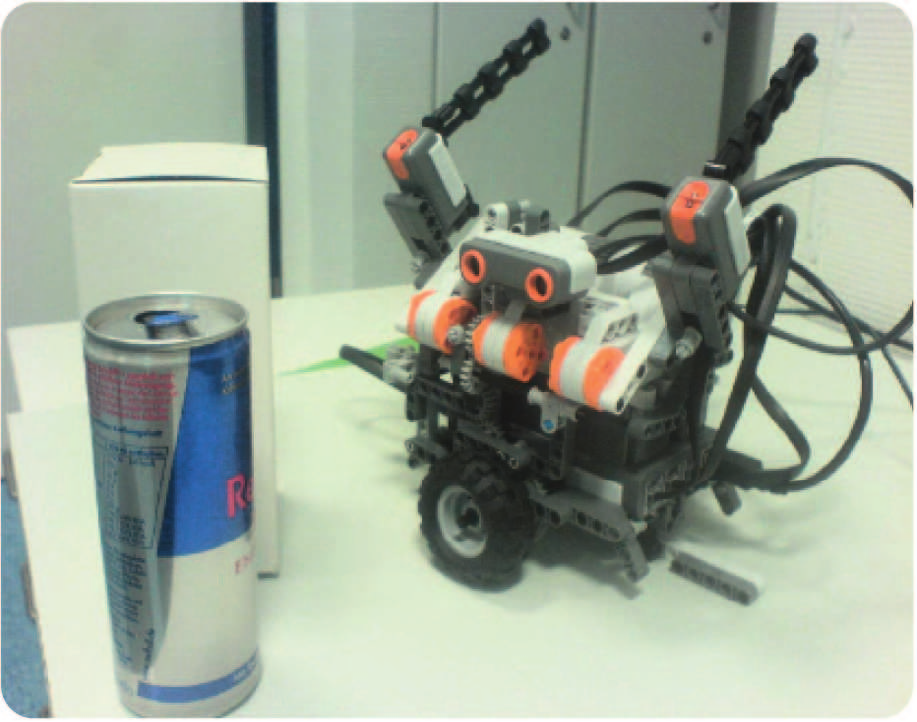
\includegraphics[width=0.4\linewidth]{Figures/1_maye_robot.png}%
	\quad
		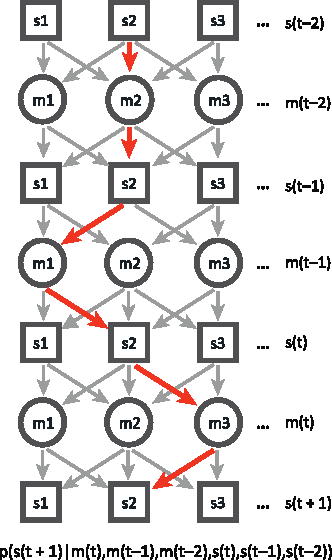
\includegraphics[width=0.18\linewidth]{Figures/1_maye_path.pdf}
	\caption{Expérimentation robotique adaptée de Engel et al. \cite[Fig.~I]{engel_wheres_2013}.
		Gauche: robot interagissant avec un objet à travers un capteur d'écho-localisation et des bras articulés.
		Droite: séquence d'expériences sensorimotrices permettant au robot de reconnaitre l'objet. 
	}
	\label{fig:maye}
\end{figure}

Certaines études considèrent la construction d'un modèle mental du monde comme un objectif en soit pour l'agent.
Je classe les \an{benchmarks} évaluant cette capacités dans la catégorie \emph{jugement} car ils ne mesurent pas directement l'aptitude d'un agent à accomplir une tâche appliquée: c'est l'expérimentateur qui juge la qualité du \an{world model} appris.
Ce jugement se fait souvent en présupposant le format de représentation utilisé par l'agent, ce qui complique la comparaison entre agents utilisant des formats de représentation différents.

Pour comparer la construction de \an{world model} par des agents utilisant des formalismes différents, certains auteurs adoptent une approche hybride. 
Dans leur article \an{Benchmarking world-model learning} \cite{warrier_benchmarking_2025}, Archana Warrier et al. proposent \emph{WorldTest}, un \an{benchmark} destiné à évaluer l'apprentissage non supervisé d'un modèle du monde en soumettant l'agent à des tâches avec un but objectif.
WorldTest différencie un \og environnement de base \fg\ durant la phase d'apprentissage ouvert, et un \og environnement dérivé à objectif explicite \fg\ durant la phase de test, qui diffère de l'environnement de base tout en lui restant corrélé. 
Il permet d'évaluer la capacité de l'agent à généraliser à partir de l'environnement de base, en mesurant ses performance à atteindre l'objectif défini dans l'environnement dérivé, de manière indépendante du formalisme de représentation utilisé.

%identifient quatre catégories de \an{benchmarks} pour évaluer l'apprentissage d'un modèle du monde:

%\begin{itemize}[label=\scalebox{.85}{$\diamond$}]
%	\item les \an{non-interactive benchmarks} évaluent la capacité de l'agent à inférer des règles sous-jacentes à partir d'exemples et à les généraliser à de nouveaux cas. Cette catégorie rejoint la catégorie \emph{statique} mais brouille la frontière entre \emph{objectif} et \emph{jugement} en testant la qualité du modèle du monde dans des jeux de questions objectives.
%	\item les \an{representation-based approaches} évaluent les modèles du monde en imposant l'usage de formats de représentation spécifiques, tels que des graphes causaux ou des langages de prédicats. 
%	L'évaluation repose sur des mesures propres à chaque format de représentation. 
%	Ces approches sont qualifiées de \og boites blanches \fg car elles nécessitent l'analyse interne des modèles. 
%	Elles présentent l'inconvénient d'empêcher la comparaison entre différents formats de représentation.  
%	Elles se situent dans la catégorie \emph{jugement} car c'est l'évaluateur qui juge de ce qui est important dans le modèle du monde. 
%	\item les \an{benchmarks} avec récompense objective utilisés en apprentissage par renforcement tels qu'\an{Open Gymnasium} de OpenAI. Ils se situent dans la catégorie \emph{dynamique} / \emph{objectif} car le modèle du monde est évalué par son utilité à atteindre des obejctifs prédéfinis. 
%	\item les \an{unsupervised RL benchmarks} reposent sur une méthode en deux phases: une phase d'interaction et une phase de test. 
%	Dans la première, l'agent interagit sans objectif explicite; dans la seconde, il est évalué sur sa capacité à accomplir une tâche spécifique.
%	Ces benchmarks floutent la frontière entre \emph{objectif} et \emph{jugement} car le choix de la tâche de test est un acte de jugement de l'examinateur, mais la performance dans cette tâche est mesurée objectivement. 
%\end{itemize} 





\section{Conclusion (en construction)}

% Revue de "Regimes of error and the epistemology of learning: from cybernetics to large language models
La revue des méthodes de mesure de l'intelligence souligne l'importance du concept \emph{d'erreur} dans les approches d'apprentissage artificiel. 
Il y a un régime 1 selon lequel l'erreur est une distance qui doit être réduite, et un régime 2 selon lequel l'erreur est un indicateur d'un défaut d'organisation interne. 
En régime 1, ce qui compte comme erreur n'est pas découvert mais est spécifié par le concepteur. L'erreur est ce qui est défini par la loss function, l'apprentissage est ce qui la réduit.
En régime 2, l'erreur est traitée comme une indication de comment le système est organisé. 
La question du diagnostique n'est pas simplement "quelle est la distance entre le signal de sortie et la consigne", mais "quelles sont les règles, hypothèses, et décompositions qui rendent cette erreur inévitable?".
Le choix du régime n'est pas neutre d'un point de vue épistémologique.
Il arrive souvent que les deux régimes soint hybridés: on entraine un système sous le régime 1 et leurs échecs sont interprétés comme des indices pour réviser l'orgnisation interne. 
Le processus d'apprentissage set redéscriptif et reconstructif.

Piaget insiste que les structures cognitives ne sont pas réductibles à des mécanismes de controle parce qu'elles impliquent des opérations réversibles et des réorganisations qui changent ce qui compte comme équilibre (Piaget 1953)
En cybernétique la régulation par l'erreur présuppose une référence stable. En termes de développement la référence elle même peut etre transformée à travers la construcction de nouvelles coordinations. 
... les erreurs systématiques devient informatives parce qu'elles structurent ldes traces d'organisation localement incohérente. La transformation de cette organisation nécessite davantage que de corriger un signal de sortie mais aussi de changer les coordinations qui les produisent. 

%Dans son article \og \an{Beyond reward and punishment} \fg, David Deutsch conclut que: 
%\begin{quote}
%	\an{So, despite its usefulness in other applications, the programming technique of defining a testable objective and training the program to meet it will have to be dropped. Indeed, I expect that any testing in the process of creating an AGI risks being counterproductive
		%, even immoral, just as in the education of humans. 
		%I share Turing’s supposition that we’ll know an AGI when we see one, but this partial ability to recognize success won’t help in creating the successful program
%	}
%	\cite[p.~119]{deutsch_beyond_2019}.
%\end{quote}

%Voir le chapitre de Thomas Schmid pour une revue récente de l'impact des idées constructivistes sur l'AI \cite{schmid_constructivism_2023}.

Cette revue des fondements théorique conduit à penser que, si on veut comprendre l'intelligence, on doit commencer par comprendre comment se met en place le contrôle des mouvements et l'organisation des comportements. 
L'agent doit construire lui même sa connaissance à partir de son \emph{expérience} (terme utilisé par Locke) et sers impressions sensibles (terme de Hume), en s'appuyant éventuellement sur des \emph{connaissances a priori} (terme de Kant), qui, dans le cas du vivant, seraient héritées de l'évolution phylogénétique.

Pour investiguer cette question je propose un programme de recherche qui inclut les principes suivants. 


\begin{enumerate}[itemsep=0pt, parsep=0pt, partopsep=0pt]
	\item Absence de présupposés ontologique sur les entités du monde
	\item Signal sensoriel non représentationnel
	\item Socle de connaissances
	\begin{itemize}[label=\scalebox{.85}{$\diamond$}, itemsep=0pt, topsep=0pt, parsep=0pt, partopsep=0pt]
		\item Séquentialité
		\item Géométrie élémentaire
		\item Préférences comportementales
	\end{itemize}
	\item Evénements d'interaction
	\begin{itemize}[label=\scalebox{.85}{$\diamond$}, itemsep=0pt, topsep=0pt, parsep=0pt, partopsep=0pt]
		\item Schèmes sensorimoteurs
		\item Valence motivationnelle
	\end{itemize} 
	\item Environnement ouvert
	\begin{itemize}[label=\scalebox{.85}{$\diamond$}, itemsep=0pt, topsep=0pt, parsep=0pt, partopsep=0pt]
		\item Absence de récompense extrinsèque
		\item Motivation intrinsèque
		\item Etats du monde initialement inconnus
	\end{itemize} 
	\item Apprentissage constructiviste
	\begin{itemize}[label=\scalebox{.85}{$\diamond$}, itemsep=0pt, topsep=0pt, parsep=0pt, partopsep=0pt]
		\item Apprentissage hiérarchique \an{bottom-up}
		\item Génération de micro hypothèses
		\item Révocation des hypothèses non validées par l'expérience
	\end{itemize} 
	\item Construction de sens pragmatique
	\begin{itemize}[label=\scalebox{.85}{$\diamond$}, itemsep=0pt, topsep=0pt, parsep=0pt, partopsep=0pt]
		\item Ancrage dans l'expérience sensorimotrice
		\item Lié aux préférences comportementales
	\end{itemize} 
	\item Benchmarsk dynamique / jugement
	\begin{itemize}[label=\scalebox{.85}{$\diamond$}, itemsep=0pt, topsep=0pt, parsep=0pt, partopsep=0pt]
		\item Comportements instinctifs
	\end{itemize} 
\end{enumerate}




%Notre examen de l'apprentissage développemental naturel nous conduit à penser que le problème suivant est un problème intéressant en informatique:

Ce programme peut se résumer par concevoir un agent artificiel qui puisse:

Construire et réitérer des comportements spatio-séquentiels hiérarchiques basés sur des préférences intéractionnelles initiales
La possibilité de réitérer des comportements appris à un haut niveau hiérarchique de manière adaptée implique la capacité de construire des représentations pertinentes du monde tel que l'agent en fait l'expérience. 


...

Ce projet se situe dans le quadrant supérieur droit de la Figure \ref{fig:mesures}: les mesures dynamiques faisant appel au jugement humain, soit par interaction directe d'un humain avec l'agent, soit par analyse des comportements basés sur des enregistrements ou des traces. 


